\documentclass[handout, 12pt]{beamer}
%\documentclass[11pt]{beamer}

% \tiny\scriptsize\footnotesize\small\normalsize\large\Large\LARGE\huge\Huge
% Adjust interline spacing


\usepackage[latin1]{inputenc}
\usepackage{amsmath,amssymb,amsfonts,euscript,mathrsfs,wasysym,textcomp}
\usepackage{array}
\usepackage{multirow}
\usepackage{multimedia}
\usepackage{fancybox}
\usepackage{psfrag}
\usepackage{listings}
\usepackage{pdfsync} % For compiling with TextMate

\usetheme{default} 
\setbeamertemplate{navigation symbols}{}          % suppress all navigation symbols
\setbeamertemplate{blocks}[rounded][shadow=true]  % use rounded blocks (boxes), with shadows

% Show page numbers on slides
\setbeamertemplate{footline}{\begin{beamercolorbox}[right]{section in head/foot}\insertpagenumber~~~ \vskip5pt \end{beamercolorbox}}

\setbeamercovered{transparent} 

\hypersetup{colorlinks        = true,    
			linkcolor         = blue,    
			linkbordercolor   = {1 0 0},    
			urlcolor          = cyan,    
			bookmarks         = {true,},    
			bookmarksopen     = {true,},    
			bookmarksnumbered = {false,},    
			pdftitle          = {ConnectMV Courses},    
			pdfsubject        = {ConnectMV Courses},    
			pdfauthor         = {Kevin Dunn, ConnectMV},    
			pdfproducer       = {LaTeX, wiki2beamer, beamer, BeamerPDF},    
			pdfkeywords       = http://connectmv.com/,
		}
\usepackage{pgfpages}

\makeatletter
\def\hlinewd#1{%
\noalign{\ifnum0=`}\fi\hrule \@height #1 %
\futurelet\reserved@a\@xhline}
\makeatother

\definecolor{todoGreen}{rgb}{0.0, 0.9, 0.0}
\definecolor{myGreen}{rgb}{0.,0.4,0.}
\definecolor{myOrange}{rgb}{1.,0.5,0.}
\definecolor{myBlue}{rgb}{0.0,0.1,0.9}
\definecolor{myRed}{rgb}{1.0,0.0,0.0}

% Some definitions
\newcommand{\todo}[1]{{\center{\color{todoGreen} #1}}}
%\newcommand{\transp}[1]{\ensuremath{{#1}^\textnormal{\textsf{T}}}}  % transpose
%\newcommand{\RR}{\textnormal{\textsf{I}\!\textsf{R}}}  % Real number
%\newcommand{\En}[1]{\ensuremath{\RR^{#1}}}             % Real number raised to a power


\title[]{\large Latent Variable Methods for Batch Processes}
\subtitle[]{Learning from data}
\author[]{Instructor: Kevin Dunn \\{\tt kevin.dunn@connectmv.com}\\ http://connectmv.com}
\institute[]{}
\date[]{Course notes \copyright~ ConnectMV, Inc. \\ \vspace{1cm}{\footnotesize Presented at GSK, Mississauga, February 2011}}

\begin{document}
\begin{frame} \titlepage \end{frame}

% Columns
%
% 	\begin{columns}
% 		\column{.80\textwidth}
% 		\begin{exampleblock}{}
% 			\centering{In engineering applications, use \alert{double-precision or better} to mitigate the effect of round-off error}
% 		\end{exampleblock}
% 	\end{columns}
% \end{frame}
%
%  \hfill {\color{myOrange} $\leftarrow$ typical in practice!}

%-------------------------------------------------
\begin{frame}\frametitle{Outline}
\tableofcontents
\end{frame}
%-------------------------------------------------

% Day 1
% -------

% %!TEX root = batch-course.tex

%-------------------------------------------------
% Sources and resources
%-------------------------------------------------
\begin{frame}\frametitle{Sources and resources}

These notes are based on ConnectMV's experience with batch systems, but also the extensive research into batch data analysis done at McMaster University

\begin{enumerate}

	\item	Nomikos, ``Statistical Process Control of Batch Processes'', Ph.D thesis, McMaster University, 1995, {\scriptsize http://digitalcommons.mcmaster.ca/opendissertations/1667/}
	
	%\item	Garcia-Mu\~noz, ``Batch process improvement using latent latent variable methods'', Ph.D thesis, McMaster University, 2004 {\scriptsize http://digitalcommons.mcmaster.ca/opendissertations/1596/}
	
	\item	Wold, Kettaneh-Wold, MacGregor, Dunn, ``Batch Process Modeling and MSPC'', \emph{Comprehensive Chemometrics}, 2009, {\scriptsize http://dx.doi.org/10.1016/B978-044452701-1.00108-3}
		
	\item	And many other batch papers - please ask.
\end{enumerate}
\end{frame}

\begin{frame}\frametitle{}
\end{frame}

%-------------------------------------------------
\section{What do we want to learn from our data?}
%-------------------------------------------------

\begin{frame}\frametitle{What do we want to learn from our data?}

\begin{enumerate}
	\item {\bf \color{myGreen}Improve/confirm} process understanding
\begin{itemize}

	\item	confirm which phenomena have greatest effect in the data (PCA)

	\item	which variables have most influence on final quality (PLS)

	\item	interpret latent variables (all LV model types)

\end{itemize}
\end{enumerate}
\end{frame}

\begin{frame}\frametitle{What do we want to learn from our data?}

\begin{enumerate}
	\setcounter{enumi}{1}
	\item {\bf \color{myGreen}Troubleshooting}
	\begin{itemize}
		\item 	confirm a known problem occurred (SPE, \( T^2 \), \( t_a \))
		\item 	use contribution plots to diagnose
		\begin{itemize}
			\item 	what went wrong?
			\item 	when did it go wrong (batch)? 
		\end{itemize}\pause
		
		\item 	use interpretation of \( t_1, t_2 \) to explain high/low score values\pause
		\item 	use engineering judgement to fix problems from insight gained from LV outputs
	\end{itemize}
\end{enumerate}
\end{frame}
	
\begin{frame}\frametitle{What do we want to learn from our data?}

\begin{enumerate}
	\setcounter{enumi}{2}
	
	\item {\bf \color{myGreen}Improve/optimize} a process
	
	\begin{itemize}
		\item 	how can we move in the latent variable space?
		
		\item 	what causal variables can be adjusted to move in \( t_1, t_2, \ldots \)
		
		\item 	latent variable DOE's to fill in gaps in ``sparse'' models
	\end{itemize}	
	
	These all rely on the concept of \alert{``model inversion''}
	
\end{enumerate}
\end{frame}

\begin{frame}\frametitle{What do we want to learn from our data?}

\begin{enumerate}
	\setcounter{enumi}{3}
	
	\item {\bf \color{myGreen}Predictive modelling} 
	
	\begin{itemize}
		\item 	uses PLS models
		
		\item 	e.g. inferential sensors provide real-time prediction of \( \mathbf{Y} \), our final quality attributes (FQAs)
		\begin{itemize}
			\item 	PLS handles colinearity, missing values, noisy \( \mathbf{X} \)-variables
			\item 	these 3 issues cannot be dealt with by ordinary least squares
		\end{itemize}
	\end{itemize}	
\end{enumerate}
\end{frame}

\begin{frame}\frametitle{What do we want to learn from our data?}

\begin{enumerate}
	\setcounter{enumi}{4}
	\item {\bf \color{myGreen}Process monitoring} 
	
	\begin{itemize}
		
		\item 	build a model from ``in control'' operation: make sure we remain there
		
		\item 	don't need to take extra action if we remain in that space
		
		\item 	do adjust process if trending out of space; we can monitor: 
		
		\begin{itemize}
			\item 	SPE, 
			
			\item	\( T^2 \)
			
			\item	\( t_a \) score limits 
			
		\end{itemize}
		
		\item 	use contribution plots to diagnose problems
	\end{itemize}	
\end{enumerate}
\end{frame}

\begin{frame}\frametitle{What do we want to learn from our data?}

\begin{enumerate}
	\setcounter{enumi}{4}
	\item 	{\bf \color{myGreen}Process monitoring} (cont'd)	

	\vspace{10pt}	
			Advantages over \emph{univariate} monitoring:
		
			\begin{itemize}
				\item 	we monitor \textbf{many} raw variables with summarized scores, SPE, and \( T^2 \)
				\item 	i.e. we actually have \emph{fewer} control charts with multivariate monitoring
				\item 	multivariate charts interpreted in the same way as univariate charts
				\item 	i.e. no extra operator training required
				\item 	ordinary Shewhart charts do not give any help with diagnosis
			\end{itemize}	
\end{enumerate}
\end{frame}

\begin{frame}\frametitle{Tools to learn from our data}

\begin{enumerate}
	\item 	\alert{Generic}: applicable to all types of processes
	\item 	\alert{Informative}: easy to use by untrained staff for decision making
		\begin{itemize}
			\item clear and quick action possible
		\end{itemize}
	\item 	\alert{Simple to implement}: straightforward calculations and fast
\end{enumerate}

\vspace{1cm}

\begin{exampleblock}{}<2->
\centering{\large{\color{myOrange} Latent variable methods meet these criteria}}
\end{exampleblock}
\end{frame}
% 
% %!TEX root = batch-course.tex
%-------------------------------------------------
\section{General multivariate review}
%-------------------------------------------------

\begin{frame}\frametitle{Justification for latent variable methods}

\begin{enumerate}
	\item	High dimensionality in data we collect, e.g. NIR spectra
			\begin{center}
				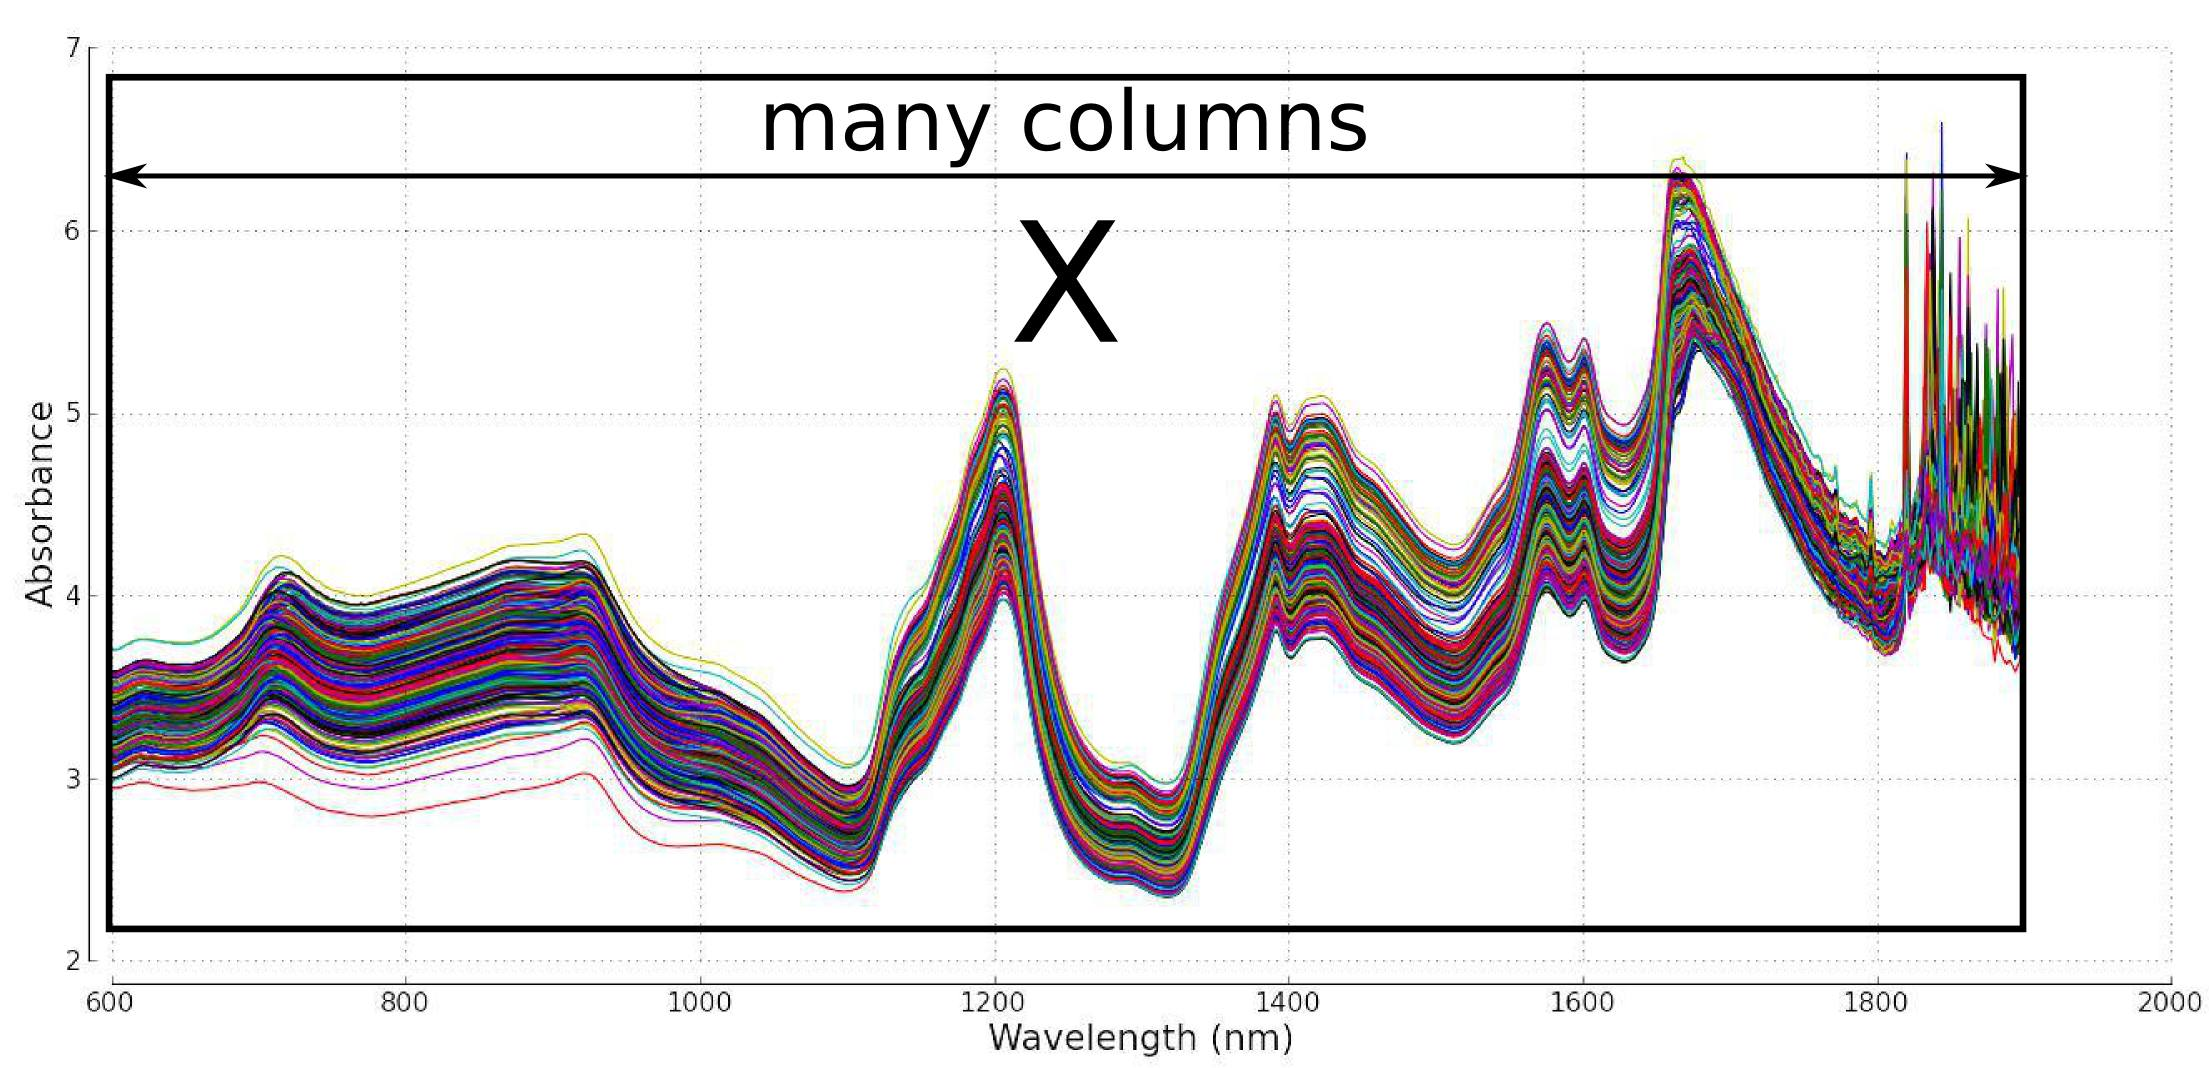
\includegraphics[width=5cm]{images/high-dimensionality-data.jpg}
			\end{center}
			
			
	\item	High correlation between the variables (duplicate info)
			\vspace{6pt}
			\begin{columns}
				\column{.30\textwidth}
				\begin{center}
					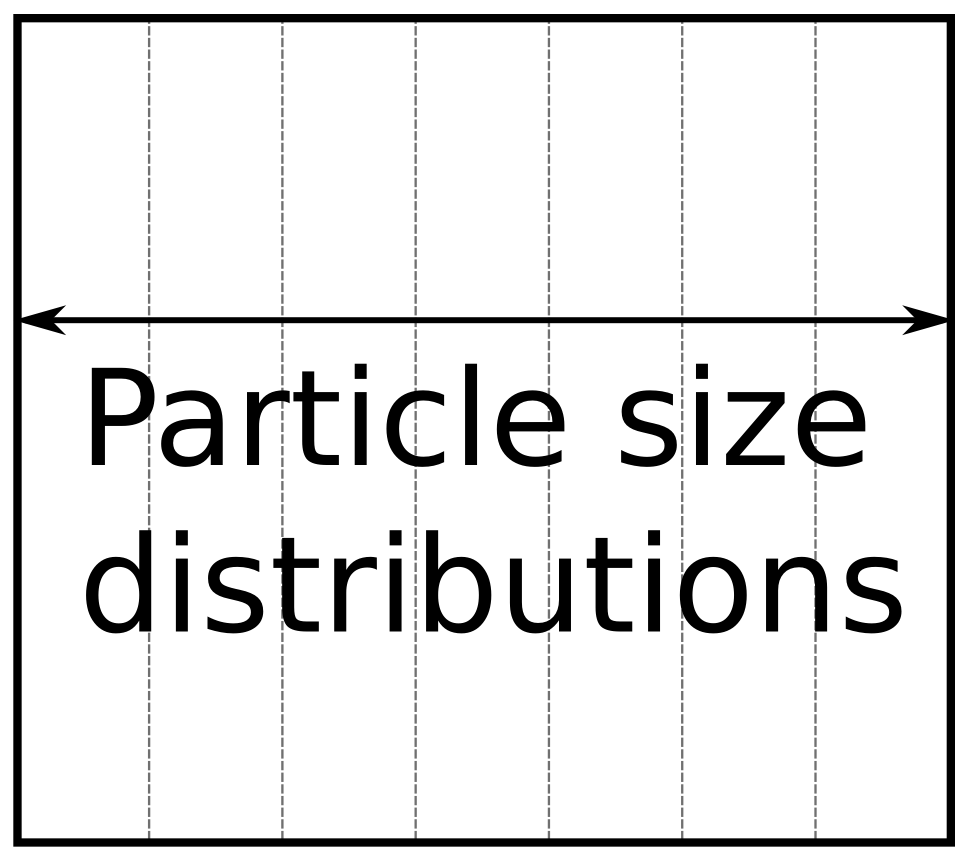
\includegraphics[width=3cm]{images/high-correlation-between-variables.png}
				\end{center}
				
				\column{.7\textwidth}
				Not a bad thing, but ordinary least squares cannot handle high correlations
				\begin{itemize}
					\item	we resort to variable selection					
					\item	we risk omitting important variables
					\item	using all data: get stronger signal from many noisy variables
					\item	batch data: highly correlated !
				\end{itemize}
				
			\end{columns}
			
\end{enumerate}
\end{frame}

\begin{frame}\frametitle{Justification for latent variable methods}

\begin{enumerate}
	\setcounter{enumi}{2}
	\item	Missing data
	
			\begin{center}
				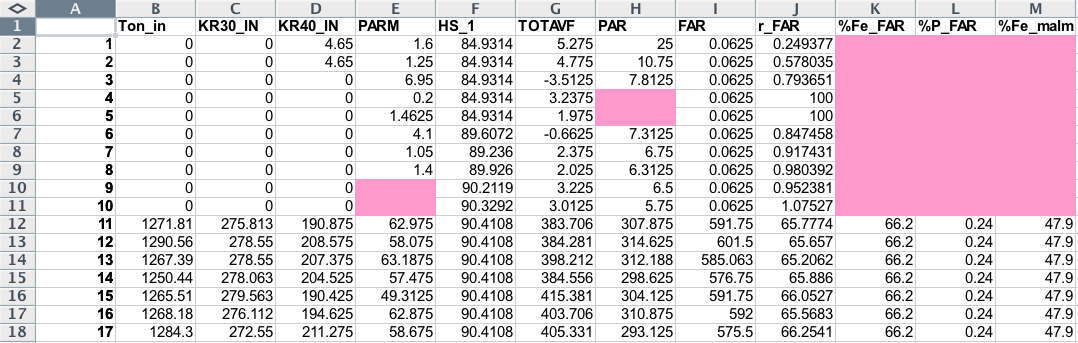
\includegraphics[width=6cm]{images/missing-data.png}
			\end{center}
			
			Batch data: usually not an issue for complete, historical batches			
			
	
	\item	Large number of samples (rows)
	
			\begin{itemize}
				\item	modern computer hardware has kept pace though
				
				\item	smart algorithms (build models from smaller data groups)
			\end{itemize} 
\end{enumerate}
\end{frame}

\begin{frame}\frametitle{Quick review of multivariate concepts: PCA}

	\begin{block}{Mathematical objective}
		PCA: find me the best summary of my data, \( \mathbf{X} \), with the fewest number of summary variables, called scores, \( \mathbf{T} \).
	\end{block}
	
	\vspace{18pt}

	\begin{center}
		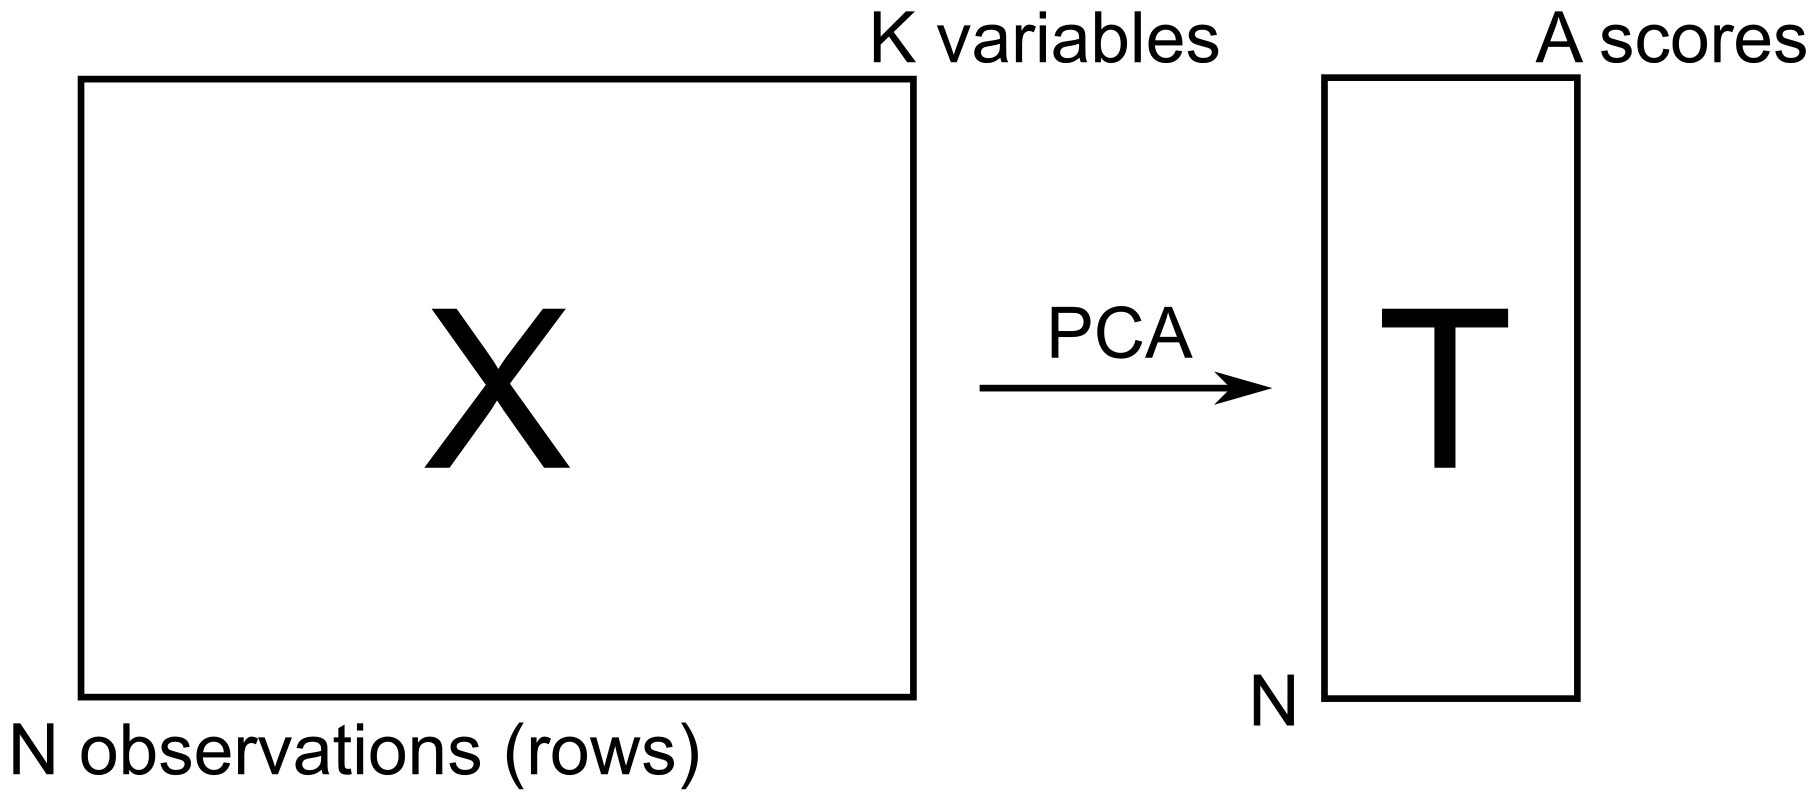
\includegraphics[width=8cm]{images/reduce-data-X-to-scores-T.png}
	\end{center}
	
\end{frame}

\begin{frame}\frametitle{What does PCA do?}

	It finds directions that best explain the data.  Also called
	
	\begin{itemize}
		\item  	``directions of greatest variance''
		\item	``loadings and scores''
		\item	``components''
		\item	``latent variables'' (LVs)
	\end{itemize}

	\begin{center}
		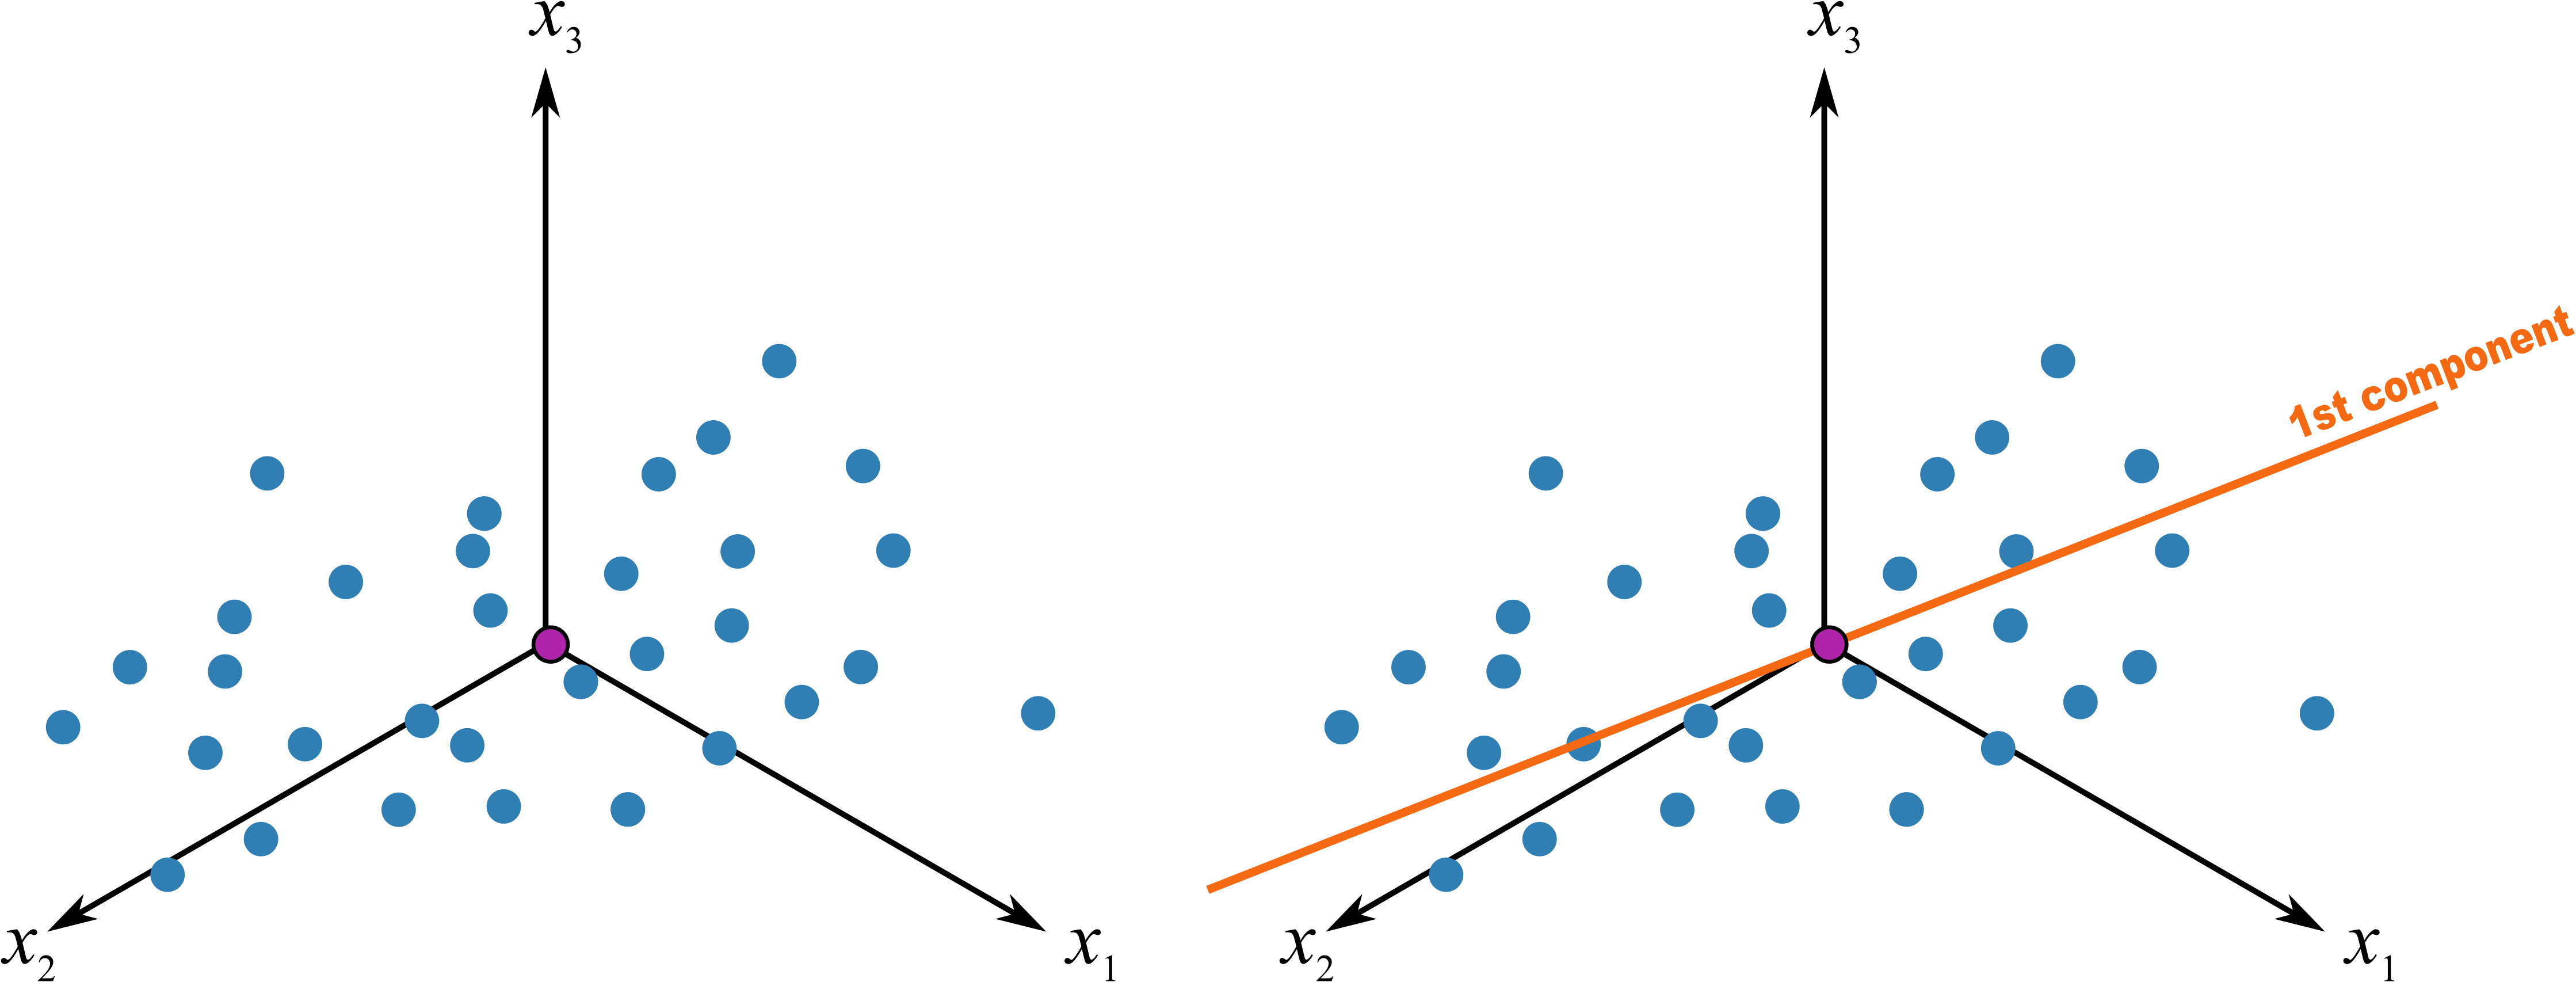
\includegraphics[width=\textwidth]{images/geometric-PCA-3-and-4-centered-with-first-component.png}
		% images/geometric-interpretation-of-PCA.svg
	\end{center}
	
	PCA finds the LVs so that LV1 explains more than LV2, which explains more than LV3, \emph{etc}.
\end{frame}

\begin{frame}\frametitle{What is a latent variable?}

	\textbf{\emph{Example}}: your health
	
	\begin{itemize}
		\item	There isn't a single measurement of ``health''.  It's an abstract concept: 
		
				\begin{itemize}
					\item	blood pressure, cholesterol, blood sugar, temperature, heart rate \emph{etc}
				\end{itemize}				
				
		\item	combine these values in some way (by a trained professional) to come up with some level of ``health''
	\end{itemize}
	
	\pause
	
	{\color{myGreen}{We can do this with any system!}}
\end{frame}

\begin{frame}\frametitle{What is a latent variable?}

	\textbf{\emph{Example}}: room temperature measured at 4 points
	
	\begin{center}
		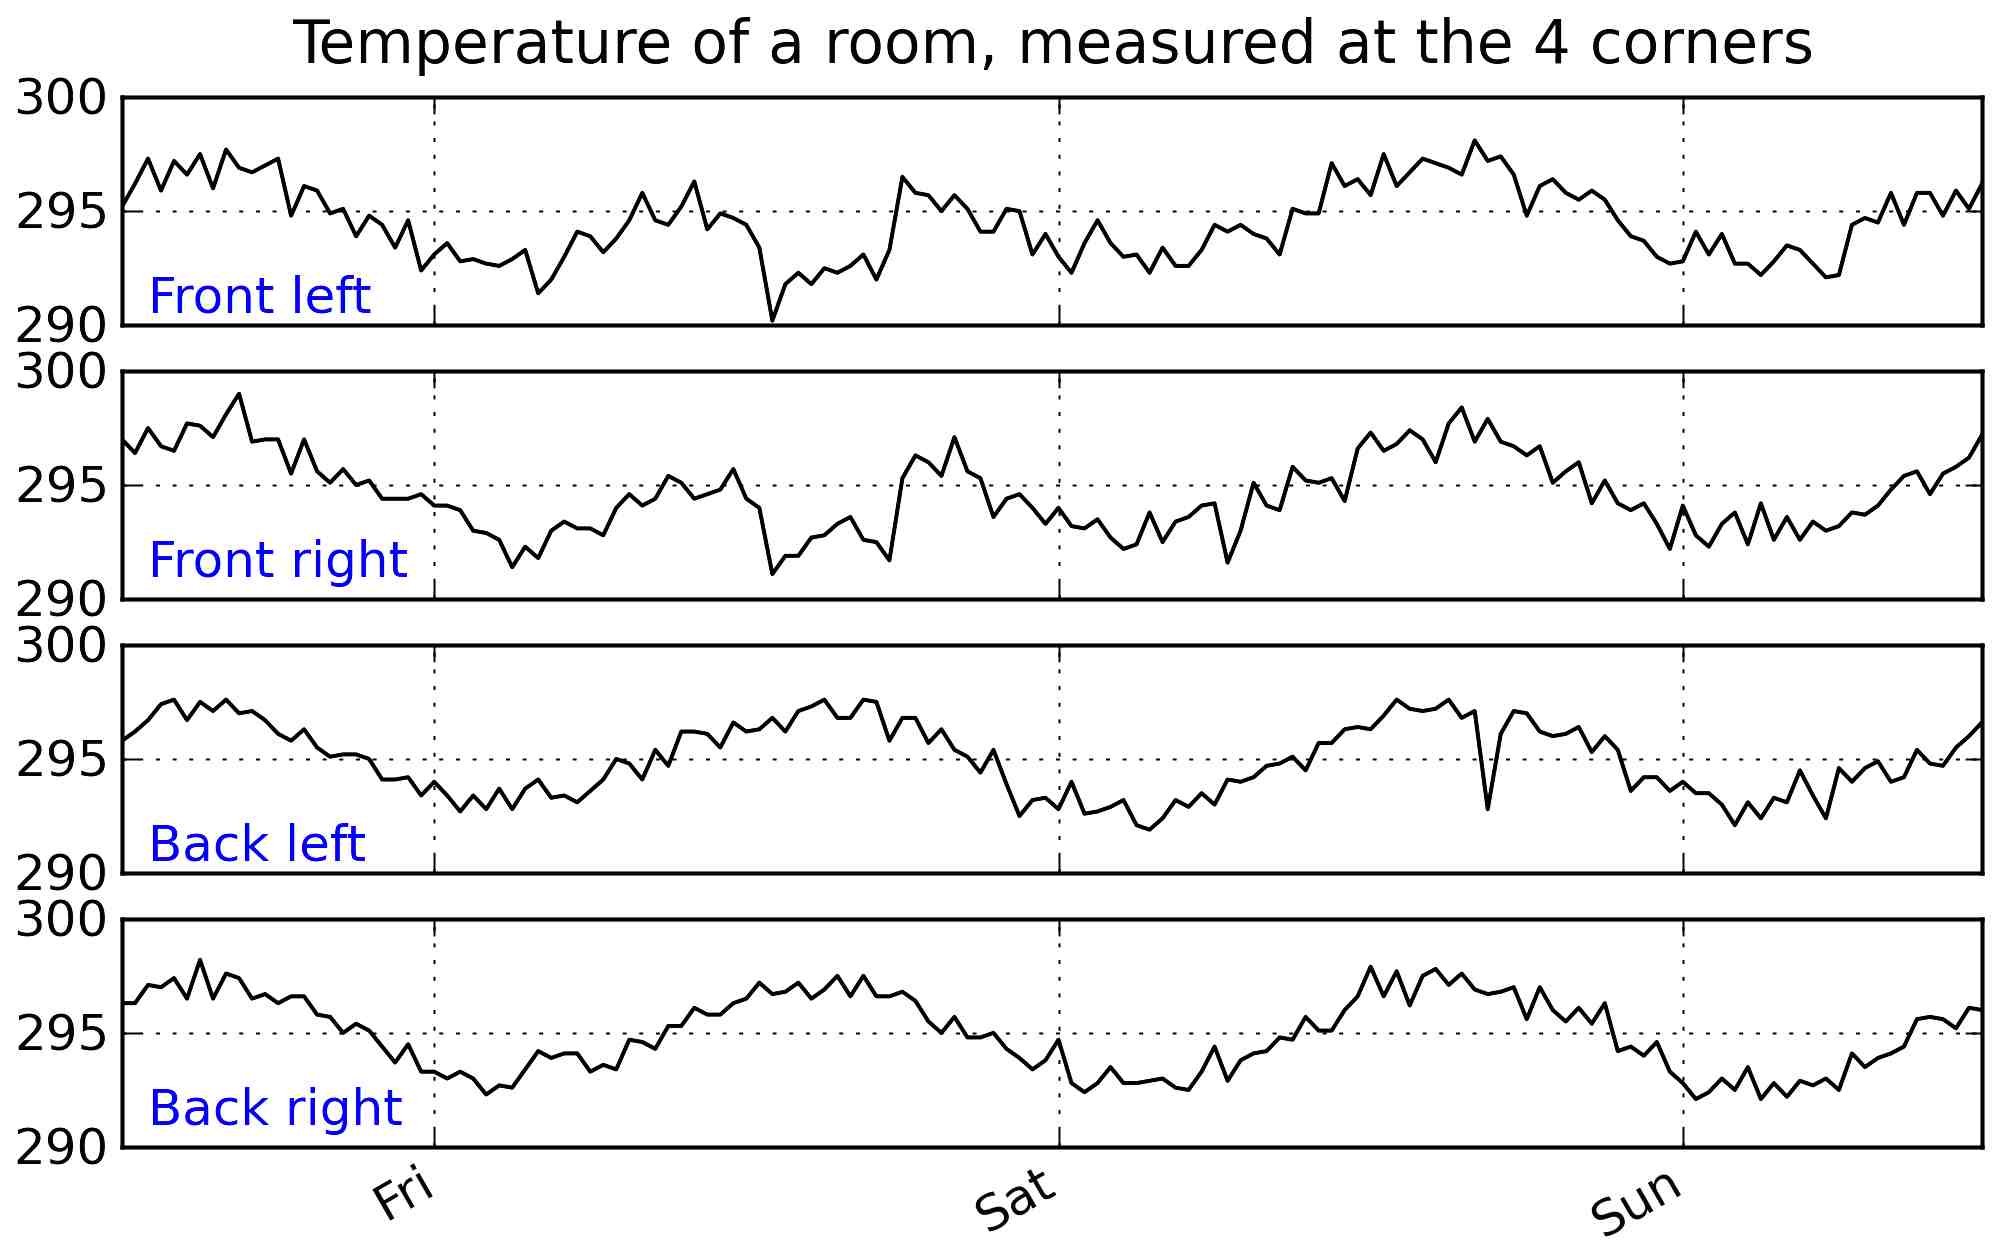
\includegraphics[width=6cm]{images/room-temperature-plots.jpg}
		% images/room-temperature-plots.py ---> PNG ---> cropped ---> saved as JPG
	\end{center}
	
	\begin{itemize}
		\item	a single phenomenon occurring, so \textbf{not 4 independent}  measurements
		
		\item	can be reduced down to 1 latent variable
		
				\begin{itemize}
					\item	just use the average
					
					\item	that's exactly what PCA does in this example
					
					\item	\( p_1 = [0.25,  0.25, 0.25, 0.25 ] \), and then scaled
				\end{itemize}
		
	\end{itemize}
	
	
	% FUTURE: come back to pencil notes in Red McMaster Sketchbook binder and add the part that shows the weighted sum calculation for the scores

\end{frame}

\begin{frame}\frametitle{LV model outputs}

	\textbf{\emph{Example}}: room temperature measured at 4 points (contd)
	
	\begin{itemize}
		
		\item	How well did PCA do with 1 latent variable? Use \( R^2 \)
		
		\item	\vspace{6pt}\( R^2 = \frac{\displaystyle\text{Variability explained in}\,\, \hat{\mathbf{X}}}{\displaystyle \text{Variability started off with}} \) \vspace{6pt}
		
		\item	The part \emph{not explained}: called the error, \( \mathbf{E} \)
	\end{itemize}
	
	\begin{center}
		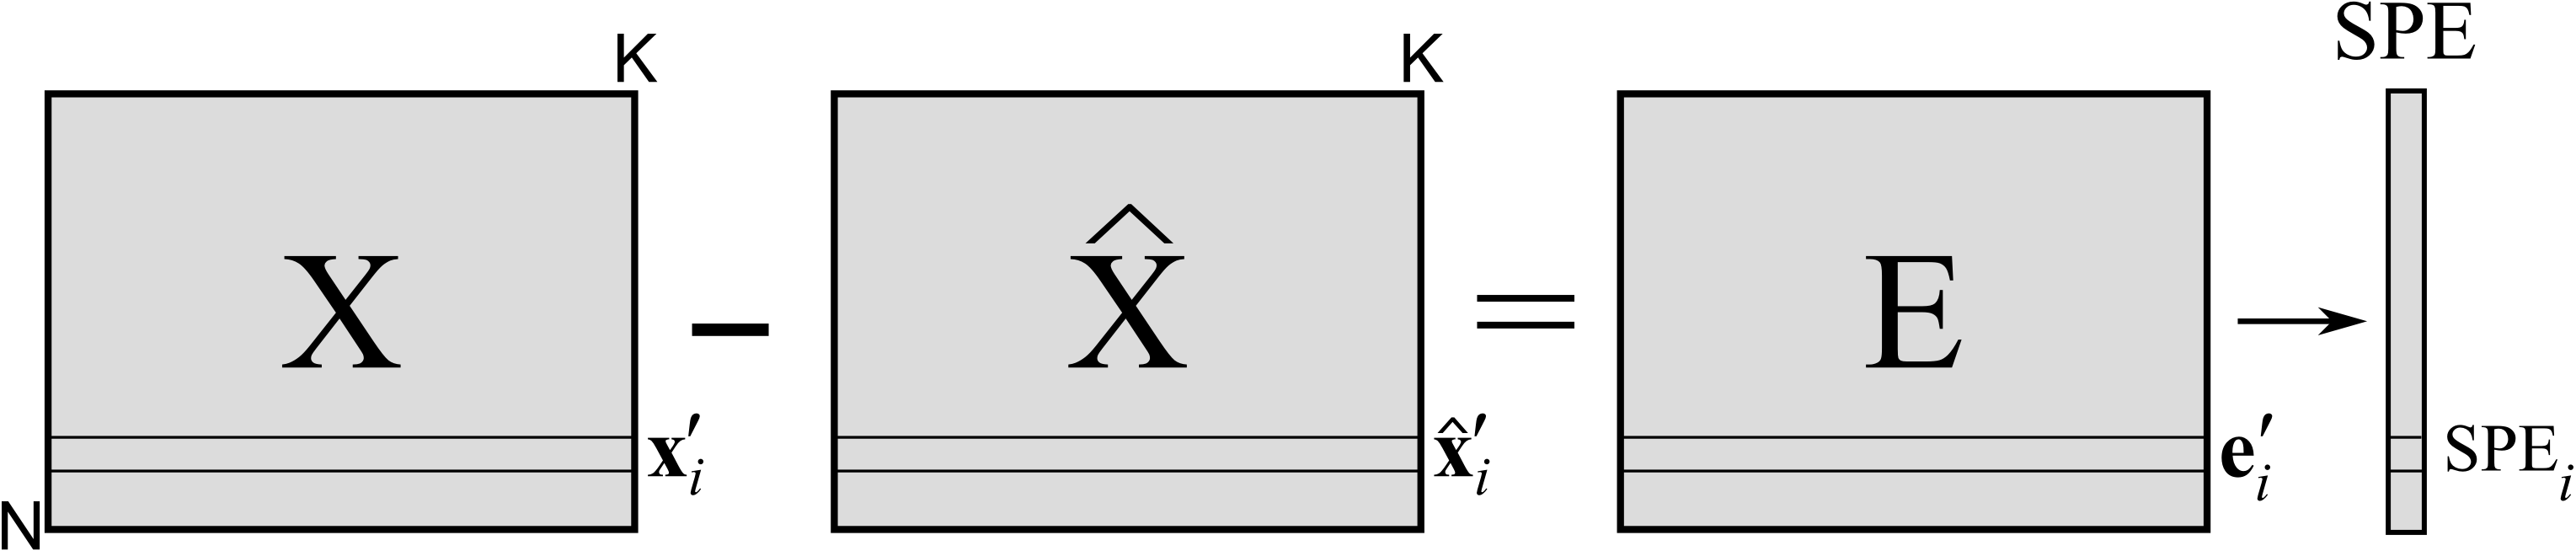
\includegraphics[width=\textwidth]{images/SPE-illustration.png}
	\end{center}

	\begin{itemize}
		\item	One SPE value per observation (row)
	\end{itemize}
	
\end{frame}

\begin{frame}\frametitle{LV model outputs}

	\textbf{\emph{Example}}: room temperature measured at 4 points (contd)
	
	\begin{center}
		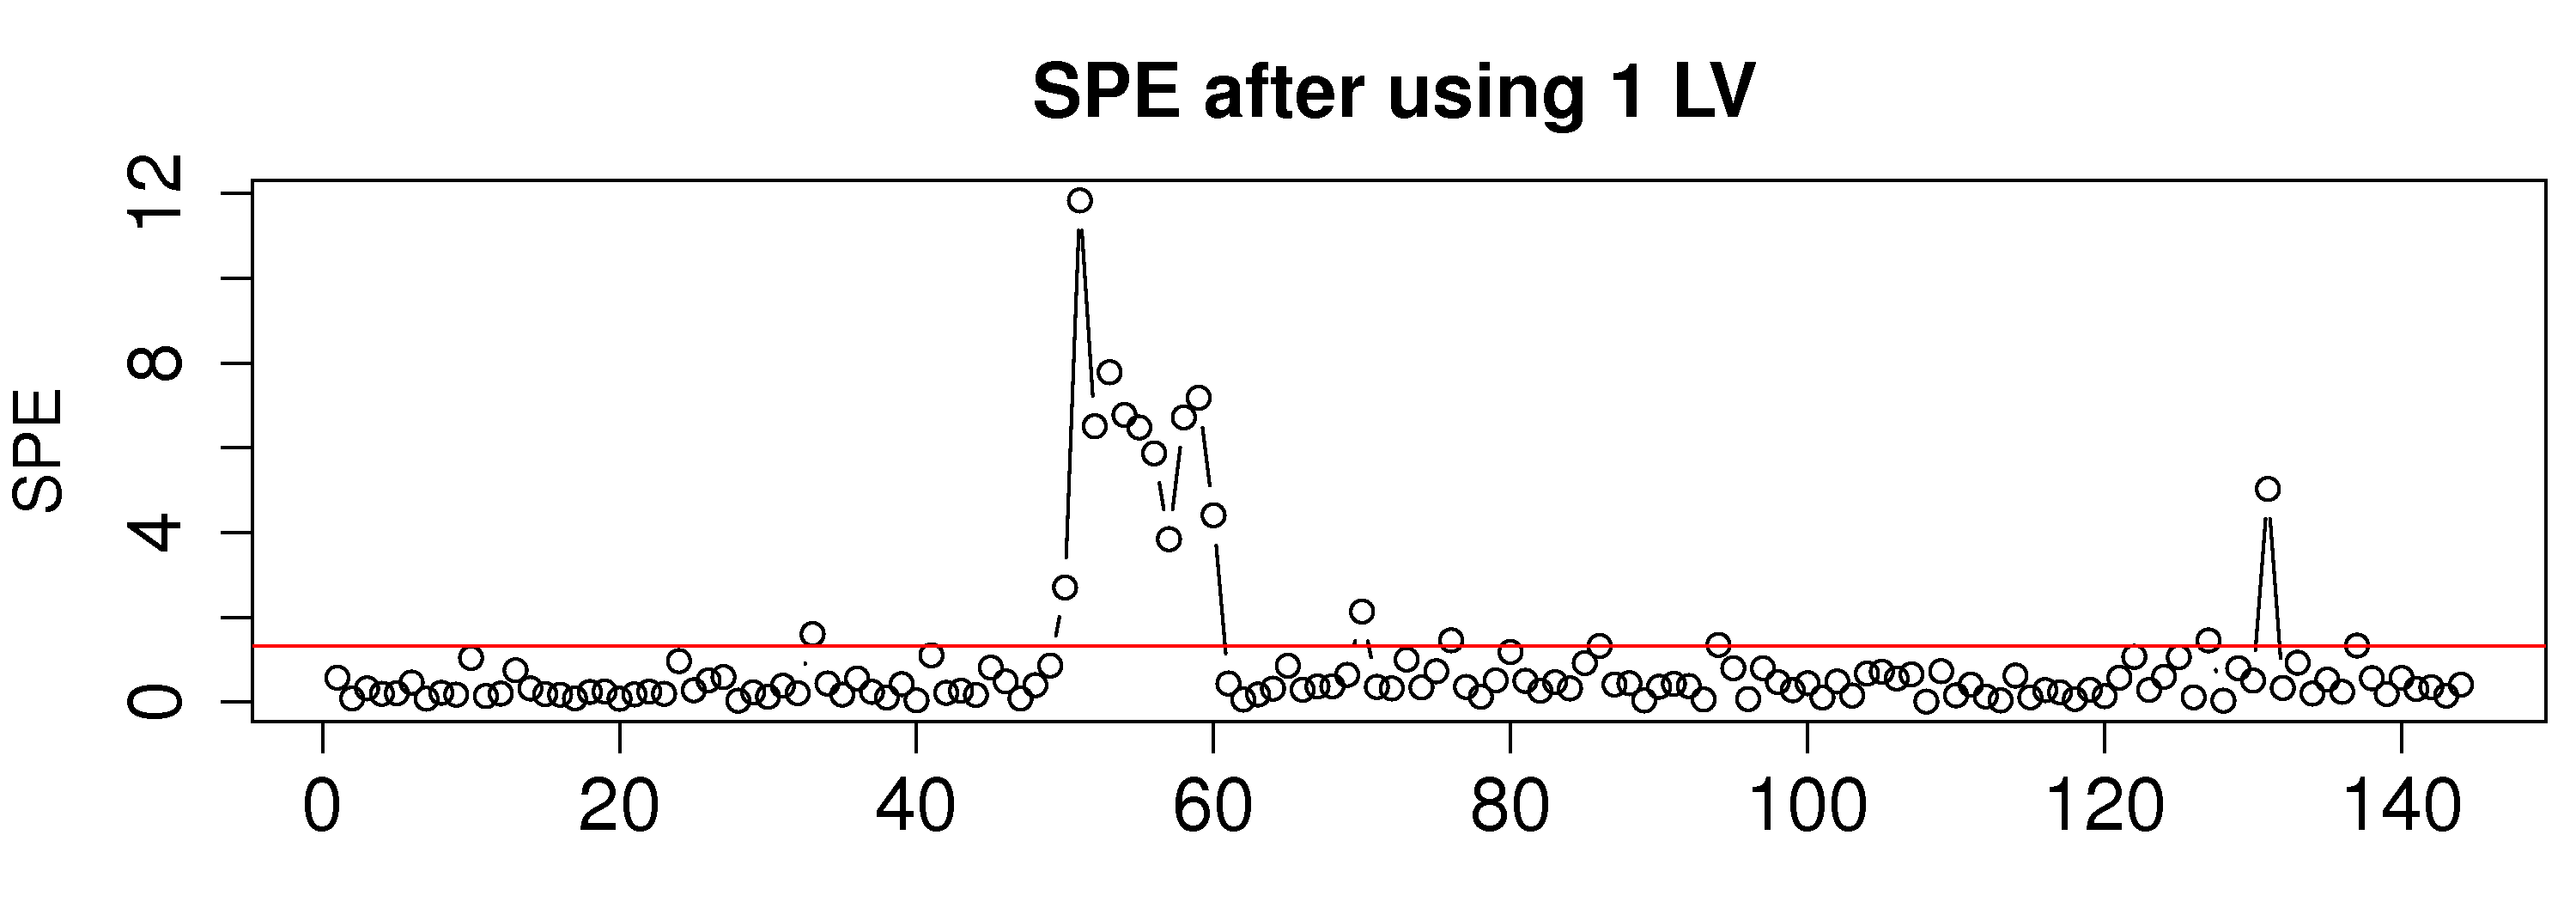
\includegraphics[width=\textwidth]{images/temperatures-SPE-after-one-PC.png}
		% From: /Users/kevindunn/ConnectMV/pid-book/latent-variable-modelling/images/temperature-data.R
	\end{center}

	Use SPE to:
	\begin{itemize}
		\item	verify whether there are unexplained phenomena: add another component to capture
		
		\item	highlight outliers, which are also just unexplained, and unusual phenomena, but few
	\end{itemize}
	
\end{frame}

\begin{frame}\frametitle{LV model outputs}

	\textbf{\emph{Example}}: room temperature measured at 4 points (contd)
	
	\begin{center}
		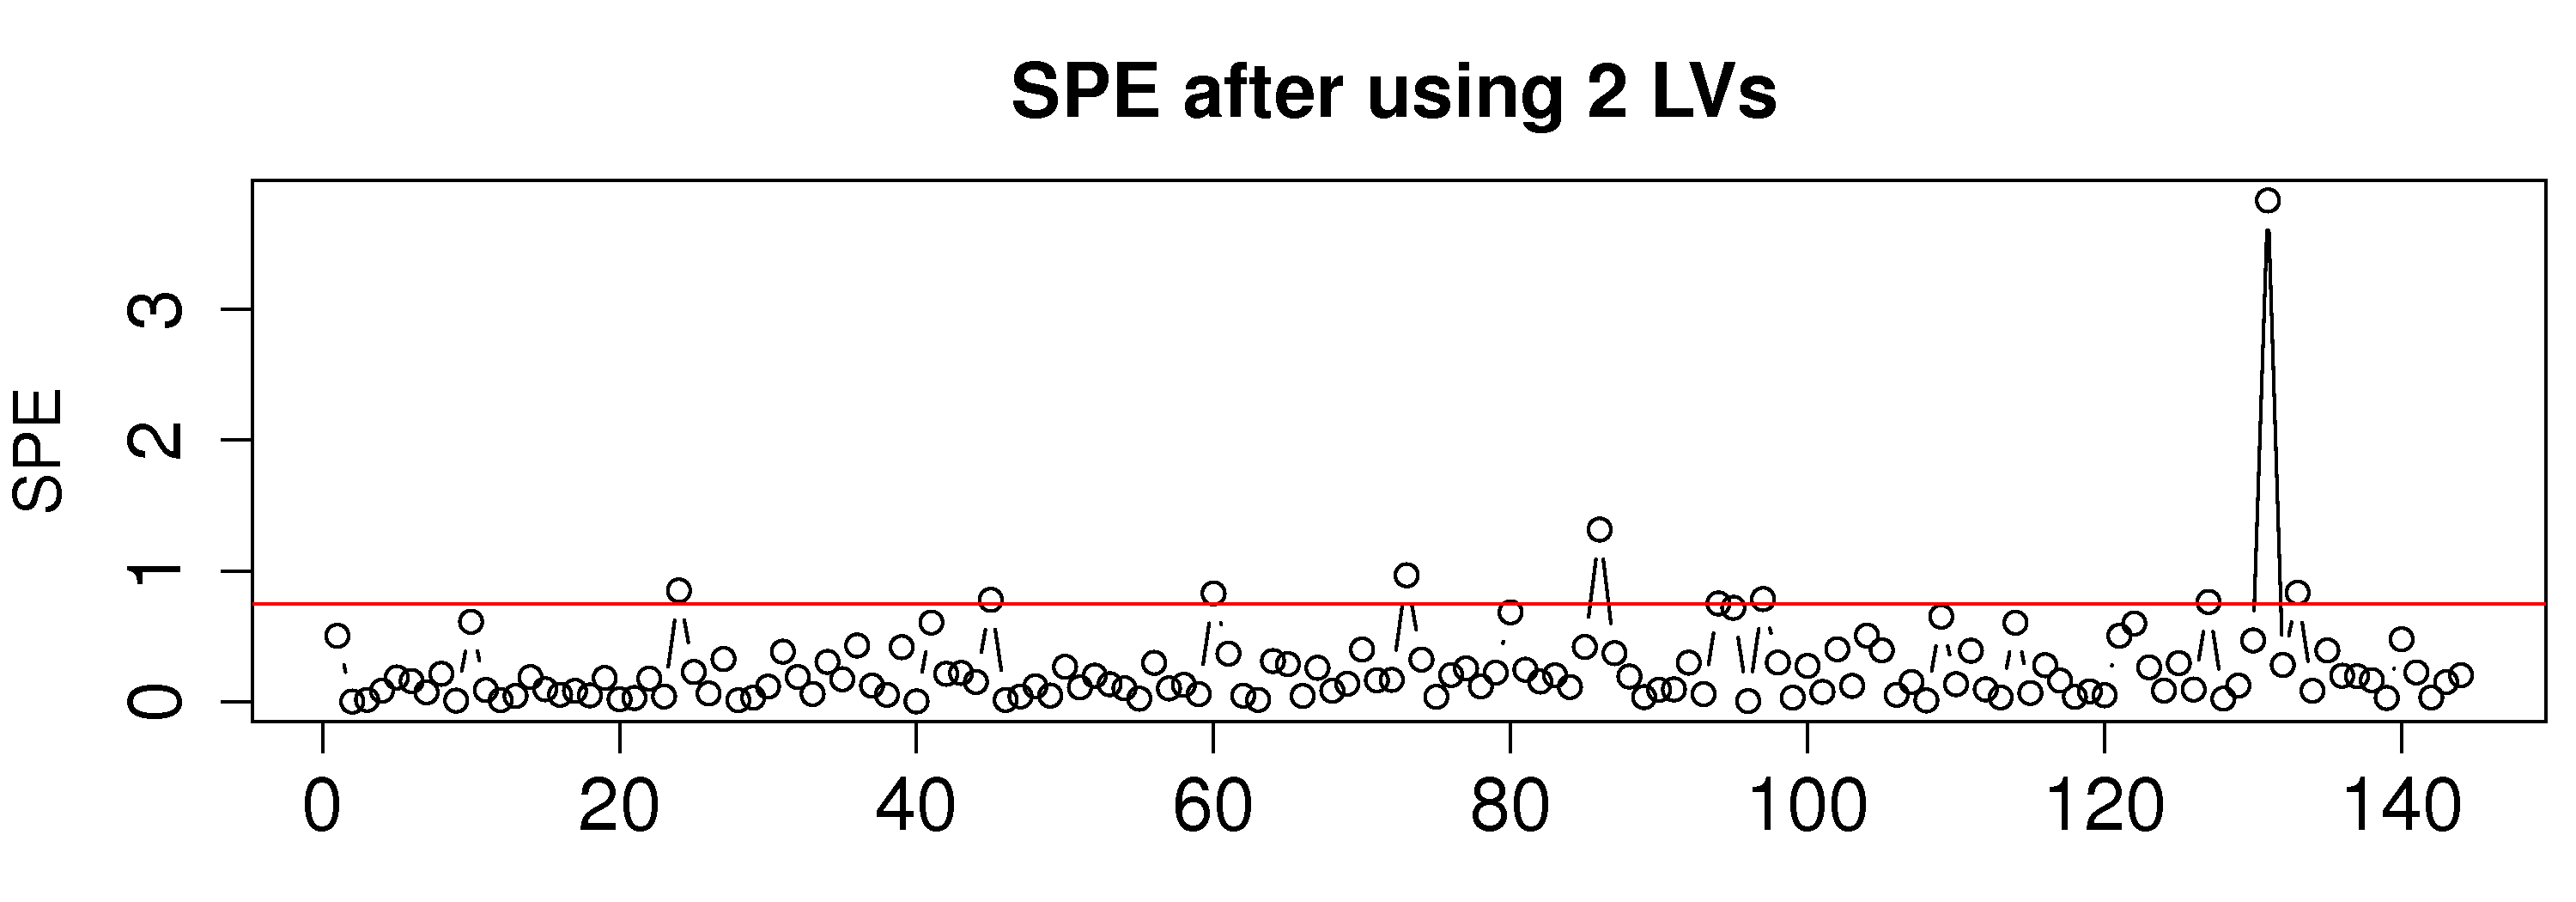
\includegraphics[width=\textwidth]{images/temperatures-SPE-after-two-LV.png}
		% From: /Users/kevindunn/ConnectMV/pid-book/latent-variable-modelling/images/temperature-data.R
	\end{center}

	\begin{itemize}
		\item	\( R^2_{a=1} = 76.6\% \)
		
		\item	\( R^2_{a=2} = 16.9\% \)
		
		\item	\( R^2_{a=1} > R^2_{a=2} > \ldots \) for PCA and PLS model
		
		\item	Every component will explain something extra
	\end{itemize}
\end{frame}

\begin{frame}\frametitle{LV model outputs}

	\textbf{\emph{Example}}: room temperature measured at 4 points (contd)
	
	\begin{itemize}
		\item	An extra phenomenon in the data was modelled: can verify this with a \( t_2 \) plot
	\end{itemize}

	\begin{center}
		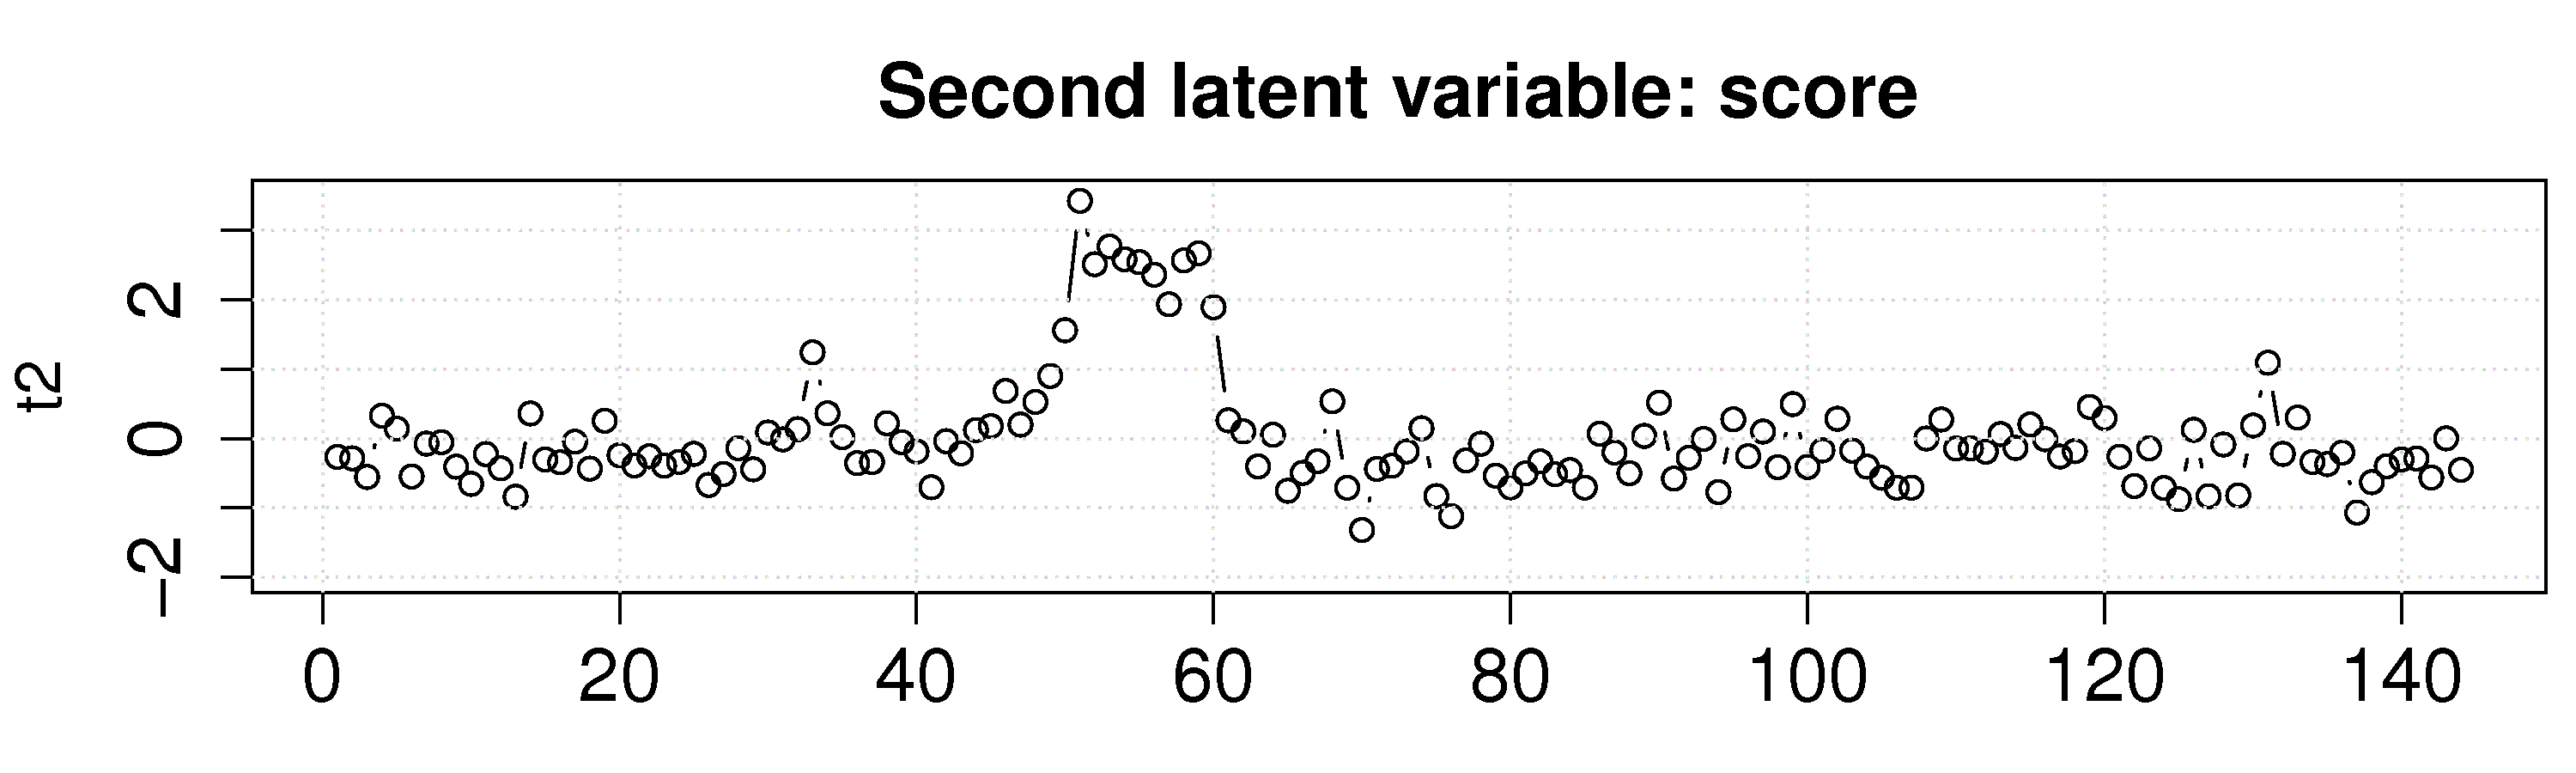
\includegraphics[width=\textwidth]{images/temperatures-LV-2-scores.png}
		% From: /Users/kevindunn/ConnectMV/pid-book/latent-variable-modelling/images/temperature-data.R
	\end{center}
\end{frame}

\begin{frame}\frametitle{Interpreting score plots: \(t_1, t_2, \ldots \)}

\begin{itemize}
	\item	Shown as scatter plot or time-series plot

	\item	Each point in plot is an observation

	\item	\(t_1\) explains more than \(t_2\); i.e. pay more attention to lower scores

		\begin{itemize}
			\item	observations that are similar appear close together in all scores
			\item	\emph{colour code} score plots by another variables: makes plot more informative
		\end{itemize}
		
	
	\item	We will make heavy use of this in batch data analysis

\end{itemize}
\end{frame}

\begin{frame}\frametitle{Interpreting loading plots: \( p_1, p_2, \ldots \)}

\begin{itemize}
	
	\item	Shown as bar plots or scatter plots

	\item 	One point per variable (tag) in the model
	
			\begin{itemize}
				
				\item	Larger loadings more important than smaller loadings
				
			\end{itemize}

	\item 	Tags that behave similarly (move together) are close together 
	
	
	\item	Batch data loadings: time-varying !  We'll see this today.
	
\end{itemize}
\end{frame}

\begin{frame}\frametitle{Quick note on data preprocessing}

\begin{itemize}
	
	\item	Columns with different units and scaling coming together in one data set
	
	\item	Scaling: gives every variable fair representation in model
	
	\item	Centering: removes arbitrary offset (usually reduces model by 1 component)
	
\end{itemize}

\begin{center}
	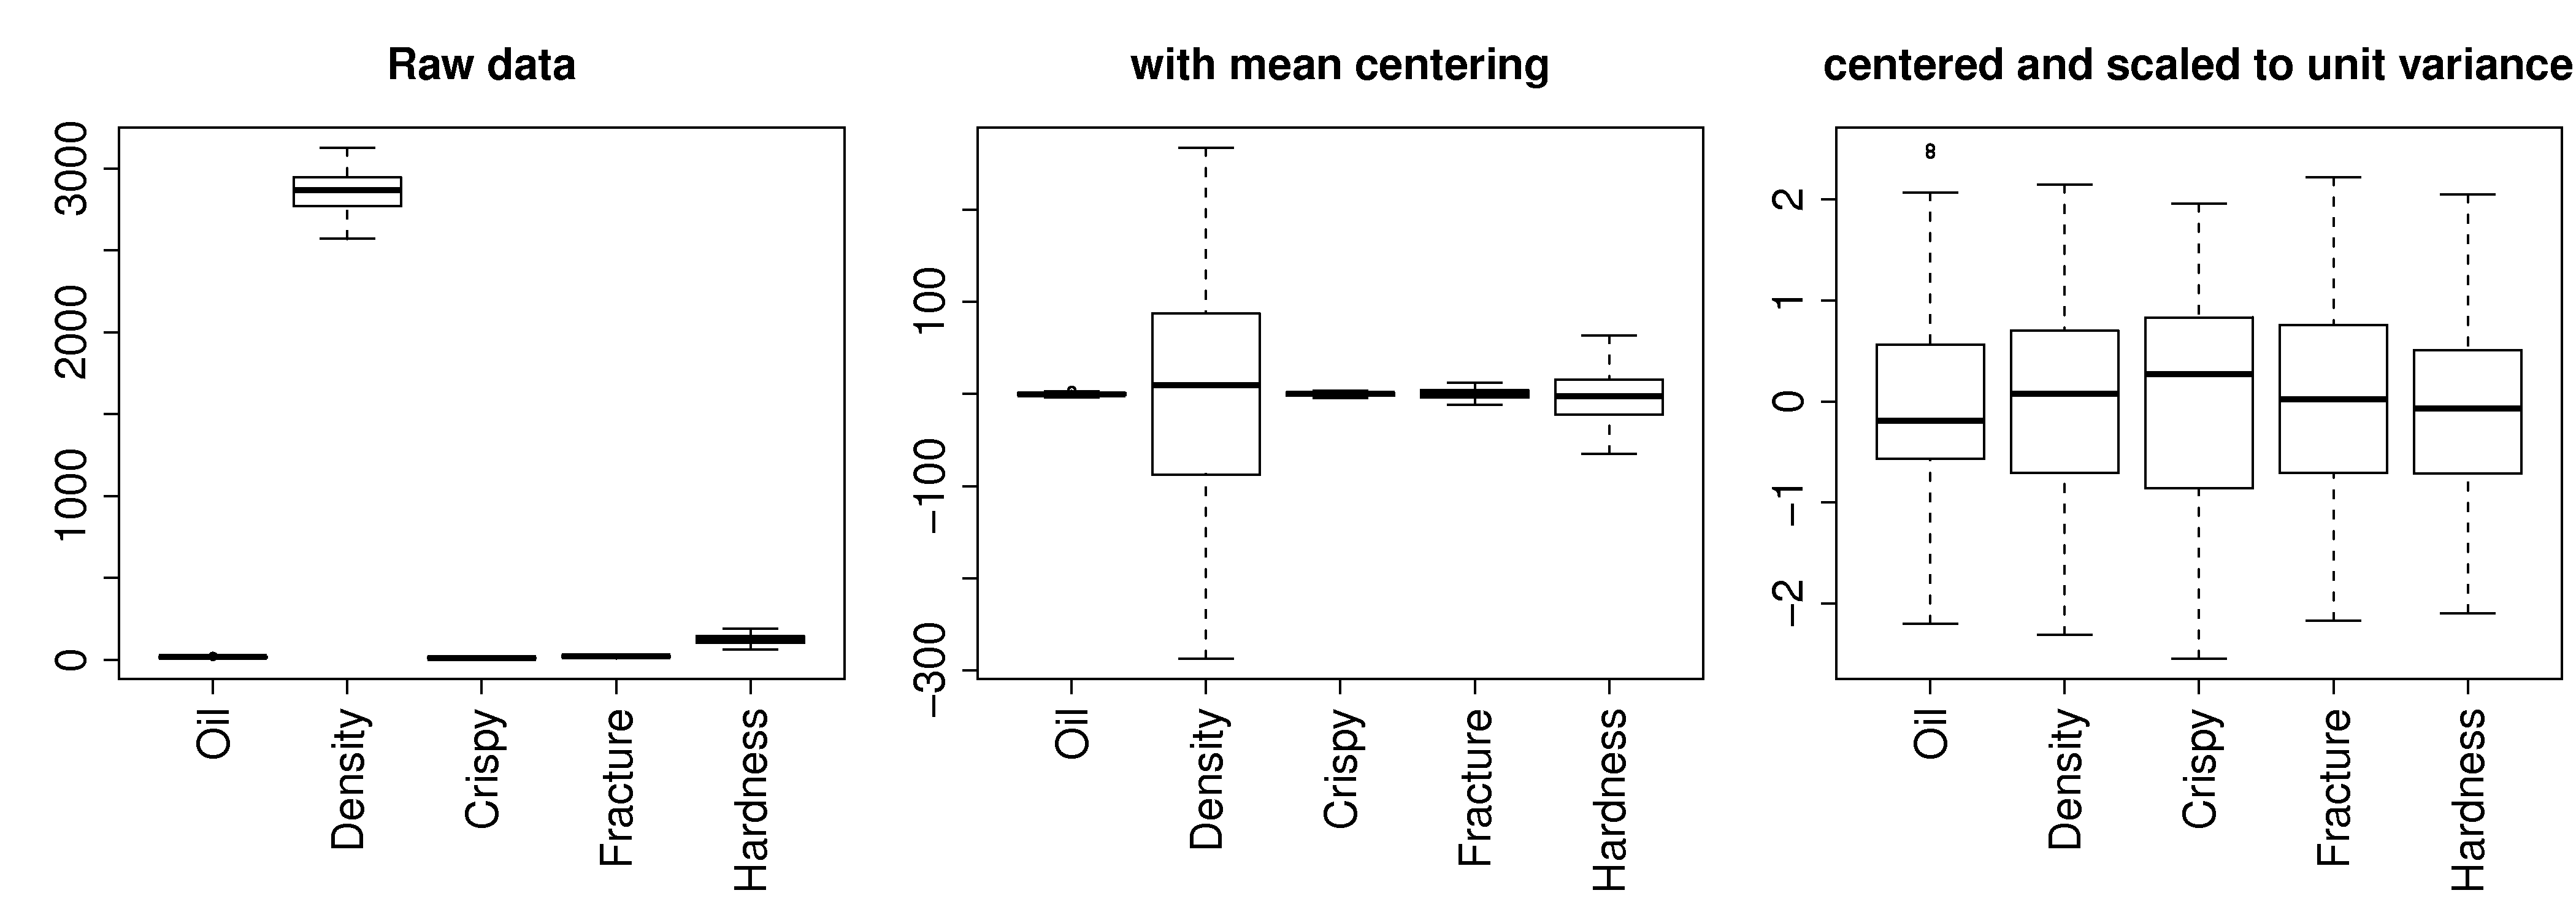
\includegraphics[width=\textwidth]{images/pca-on-food-texture-centering-and-scaling.png}
\end{center}
\end{frame}


% 
% %!TEX root = batch-course.tex
%-------------------------------------------------
\section{Batch systems}
%-------------------------------------------------
% Related concepts: phases, Z, trajectories, alignment, recipes, operators, manual steps, unfolding, charge reactor

\begin{frame}\frametitle{Batch systems: concepts and unique features}

\begin{itemize}
	\item 	Start point, an end point, and time-based evolution of tags (variables) in between 
	
	\item 	Operate essentially in open-loop i.t.o. final quality attributes (FQAs).  Basic, low-level feedback. \pause
	
	\item 	Quality measurements made afterwards, usually in a lab
	
			\begin{itemize}
				\item	used to decide batch disposition
				\item	often used to adjust next batch (batch-to-batch control)
			\end{itemize}\pause
			
	\item	Sequenced very accurately
	
	\item	Phase-based sequencing

\end{itemize}
\end{frame}

\begin{frame}\frametitle{Batch systems: concepts and unique features}

\begin{itemize}
	
	\item	Nonlinear relationship between variables; relationship changes with time \pause
	
	\item	Poor mechanistic models available (understandable)
	
			\begin{itemize}
				\item	continuous: one or two things happening all the time
				\item	batch: series of phases/events and relationships differ between (and within!) phases
			\end{itemize} \pause
			
	\item 	Past history within a batch affects the future
	
			\begin{itemize}
				\item	initial conditions: affect trajectories and FQAs								
				\item	trajectory changes from operator affect FQAs
				\item	actions taken can affect some period or all of batch, or,
				\item	even have no effect - relevant when monitoring a batch
			\end{itemize}
\end{itemize}
\end{frame}

\begin{frame}\frametitle{Batch systems: terminology for these notes}

\begin{description} 
	
	\item[ \( N \): number of batches] 
	
		\begin{itemize}
			\item	literature uses \( I \)
		\end{itemize}
		
	\item[\( K \): number of tags] 
	
		\begin{itemize}
			\item	 literature uses \( J \)
		\end{itemize}
	
	\item[\( J \): number of time steps, ] 
	
		\begin{itemize}
			\item	 literature uses \( K \)
		\end{itemize}
\end{description}

We aim for consistency with general latent variable methods: \( N \times K \times J \)

\begin{center}
	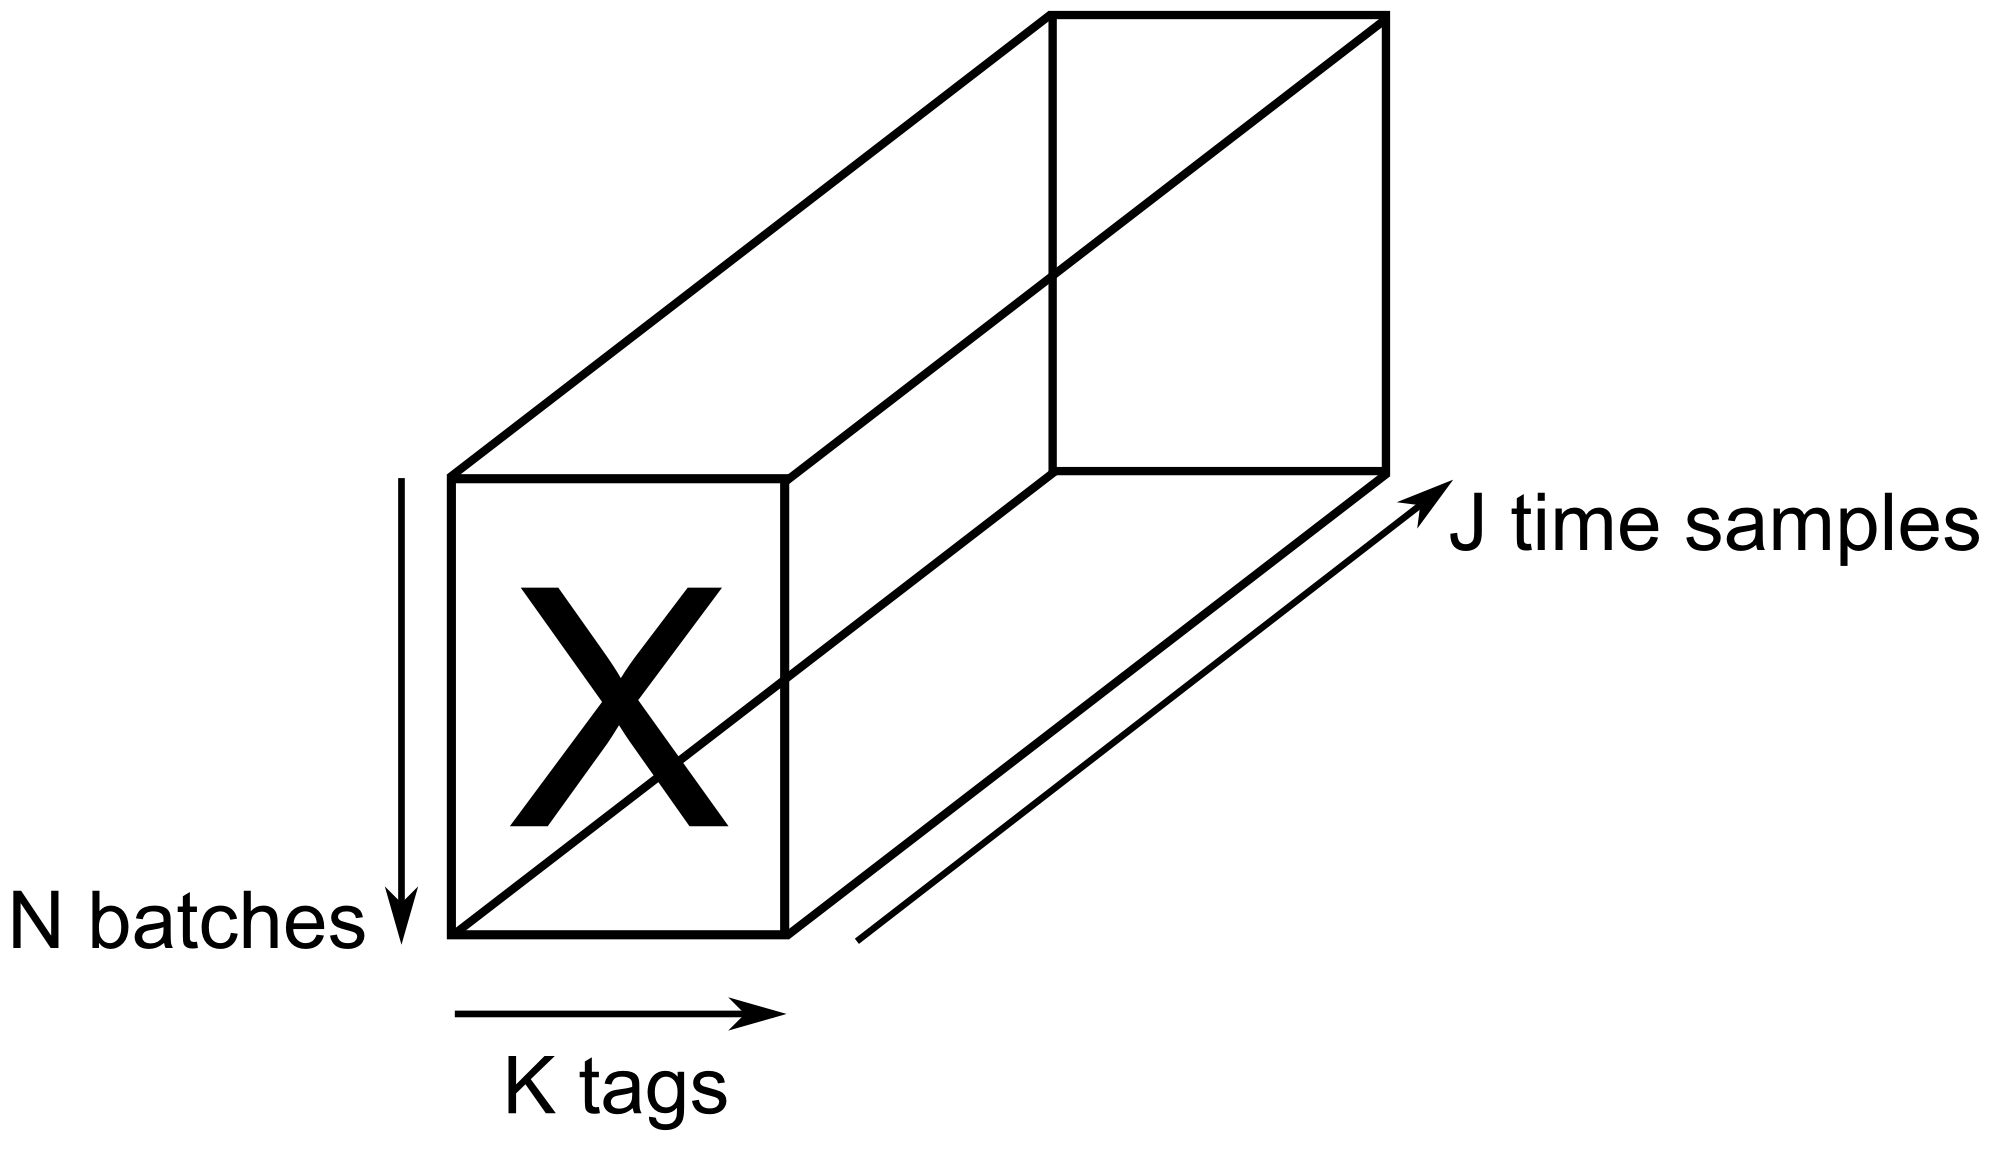
\includegraphics[width=7.2cm]{images/batch-data-cube.png}
\end{center}

\end{frame}

\begin{frame}\frametitle{Batch systems: data representation}

When retrieving batch data from computerized systems:
\begin{enumerate}
	\item	One batch per sheet in a spreadsheet, with batch ID
			
			
\includegraphics[scale=0.75]{images/batches-in-spreadsheets.png}
	
	\item	One batch per CSV file
\end{enumerate}
\end{frame}

\begin{frame}\frametitle{Batch systems: data representation}

\begin{enumerate}
	\setcounter{enumi}{2}
	\item	Stacked batches of equal duration in a single file

			\begin{center}
				
\includegraphics[width=0.9\textwidth]{images/batch-data-layers-into-page-and-unfolded-aligned}
			\end{center}
					
\end{enumerate}
The extra batch ID column is optional.  Some batch software require the data input this way.
\end{frame}

\begin{frame}\frametitle{Batch systems: data representation}

\begin{enumerate}
	\setcounter{enumi}{3}
	\item	Stacked, \textbf{but unaligned} batches, in a single file (common)
			
			\begin{columns}
				\column{.3\textwidth}
					\begin{itemize}
						\item	must also include a batch ID column

						\item	phased recipes: append a ``phase ID'' column within each batch (not shown)
					\end{itemize}
					
				\column{0.7\textwidth}
				
					\begin{center}
						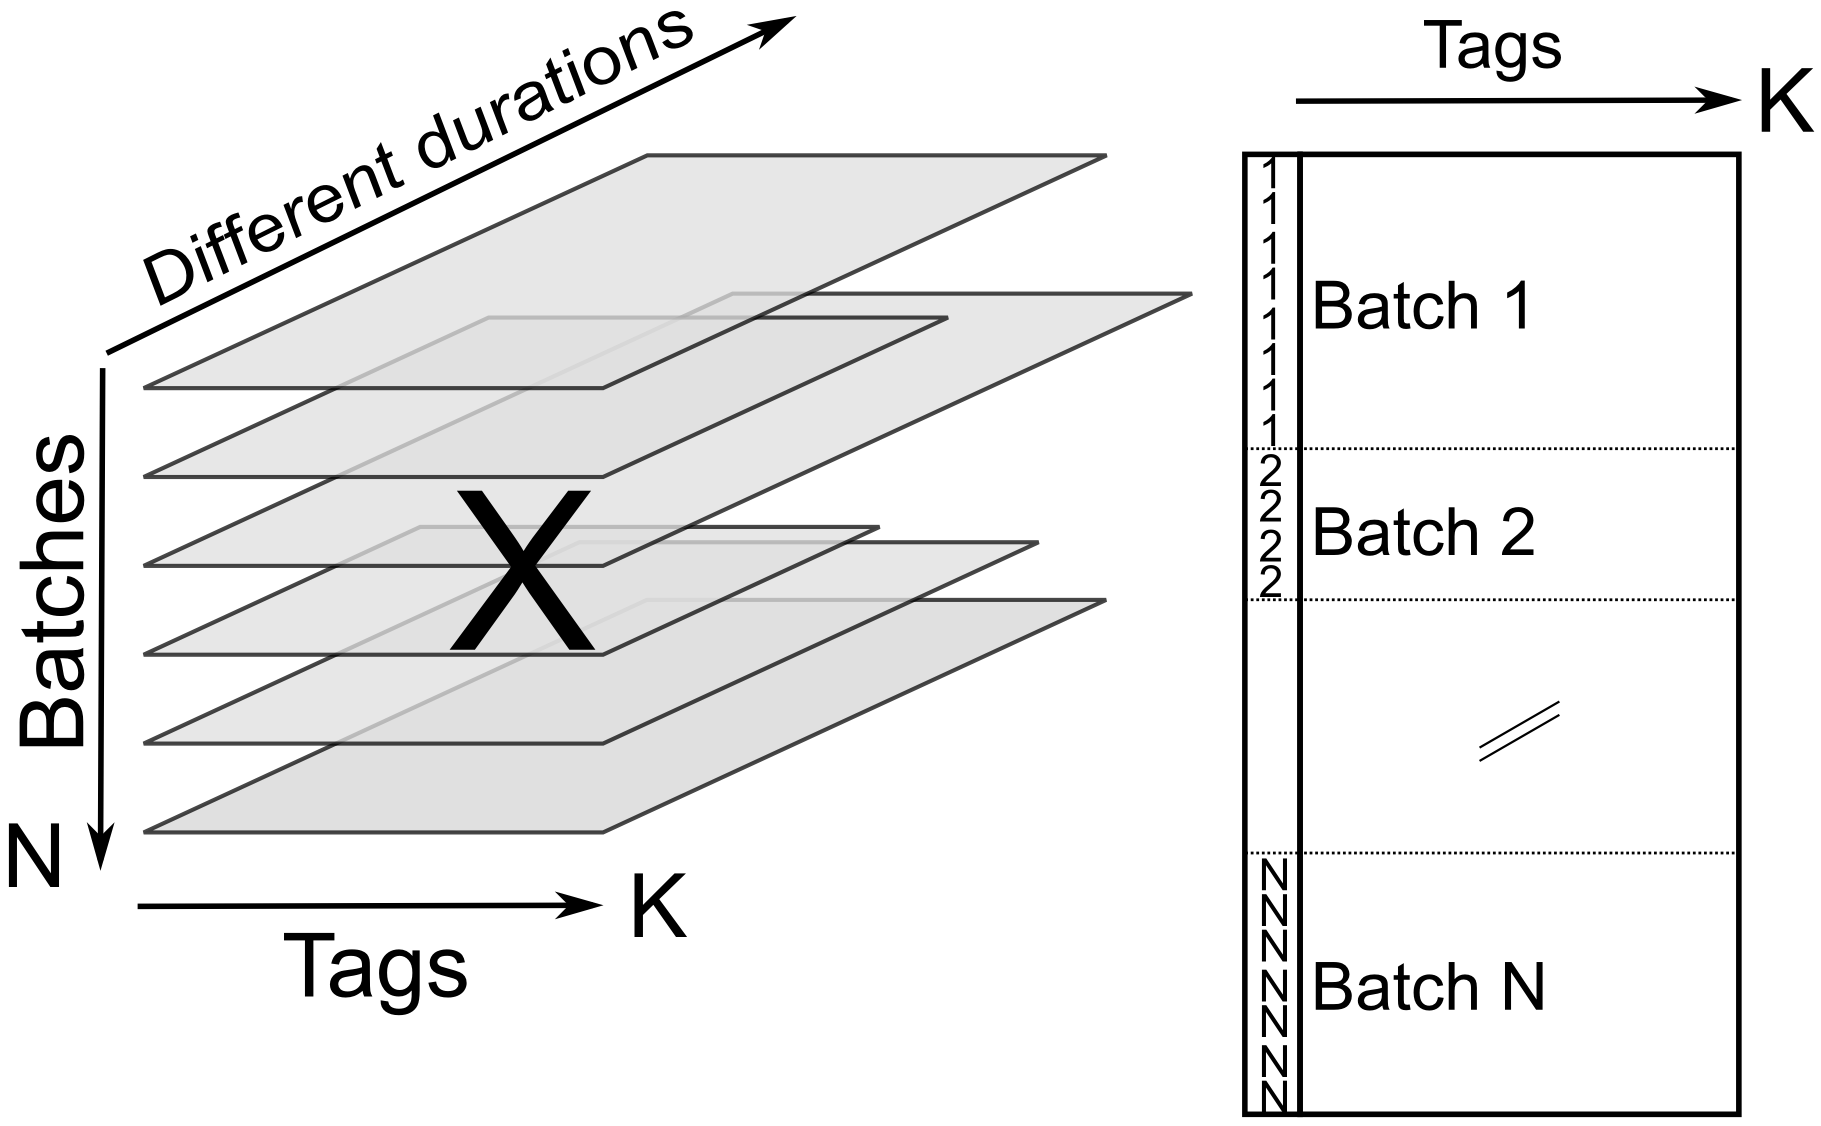
\includegraphics[width=\textwidth]{images/batch-data-layers-into-page-and-unfolded.png}
					\end{center}
					
			\end{columns}
\end{enumerate}
MATLAB can handle all the formats shown above.
\end{frame}

\begin{frame}\frametitle{Batch systems: data representation}
	
	\begin{itemize}
		\item	It is very common that the time-dimension, \( J \), is unequal	
		
		\item	We deal later with alignment: equalizing the time-dimension for all batches
	\end{itemize}
\end{frame}

\begin{frame}\frametitle{Batch systems: visualize the trajectory data}
	
	\begin{columns}
		\column{.40\textwidth}
			{\color{myOrange}{\textbf{Unaligned data}}}
 			\vfill
			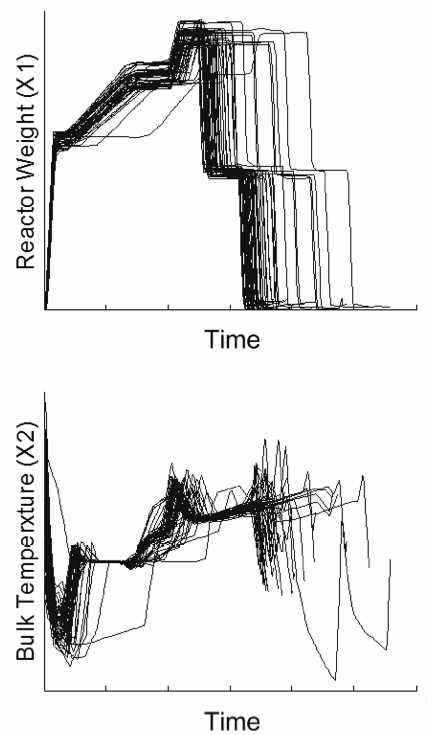
\includegraphics[height=0.8\textheight]{images/unaligned-trajectories-many-batches.png}
			% From Cecilia Rodrigues thesis, used with permission (see gmail email in February 2011)
		
		\column{.60\textwidth}
			{\color{myOrange}{\textbf{Aligned data}}}
			\vfill
			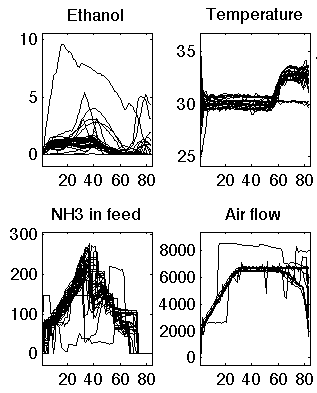
\includegraphics[height=0.8\textheight]{images/aligned-trajectories-many-batches-yeast.png}
			% Using rev 85:95b49ee15280 			
			% data = load('/Users/kevindunn/ConnectMV/Courses/Batch/datasets/yeast/yeast-data.mat');
			% b.tagNames = {'Ethanol', 'Temperature', 'Molasses', 'NH3 in feed', ...
			%               'Air flow', 'Tank level', 'pH'};
			% b.batchnames = {'rB','rC','rI','rM','rN','rQ','rR','rT','rV','rX','rZ', ...
			%                'ra','rb_1','rc_1','rd','re','rf','rg','rh','ri_1','nA', ...
			%                'tD','nG','nH','tJ','nL','nO','tP','nU','nY','rj','rk','rl'};
			% b.nBatches = 33;
			% batch_X = block(data.X, 'X', 'batch', 'tagNames', b.tagNames, 'nBatches', b.nBatches);
			% plot(batch_X, 'raw', 2, 3) % but used a limited set
	\end{columns}

\end{frame}


% 
% %!TEX root = batch-course.tex
%-------------------------------------------------
\section{Batch analysis using feature extraction}
%-------------------------------------------------

\begin{frame}\frametitle{Feature extraction methods: overview}

\begin{itemize}
	\item	Unaligned data can be a challenge (more later).
	
	\item	One alternative to alignment, if we want to get started right away: 
	
			\begin{itemize}
				\item	{\color{myOrange}{\emph{extract features}}} from each phase in each batch
				
				\item	assemble features within a row\pause
				
				\item	build ordinary PCA on \( \mathbf{X_f} \) or PLS: \( \left\{ \mathbf{Z} \,\,\text{and}\,\, \mathbf{X_f}\right\} \stackrel{\text{PLS}}{\longmapsto} \mathbf{Y} \)
			\end{itemize}
\end{itemize}

\begin{center}
	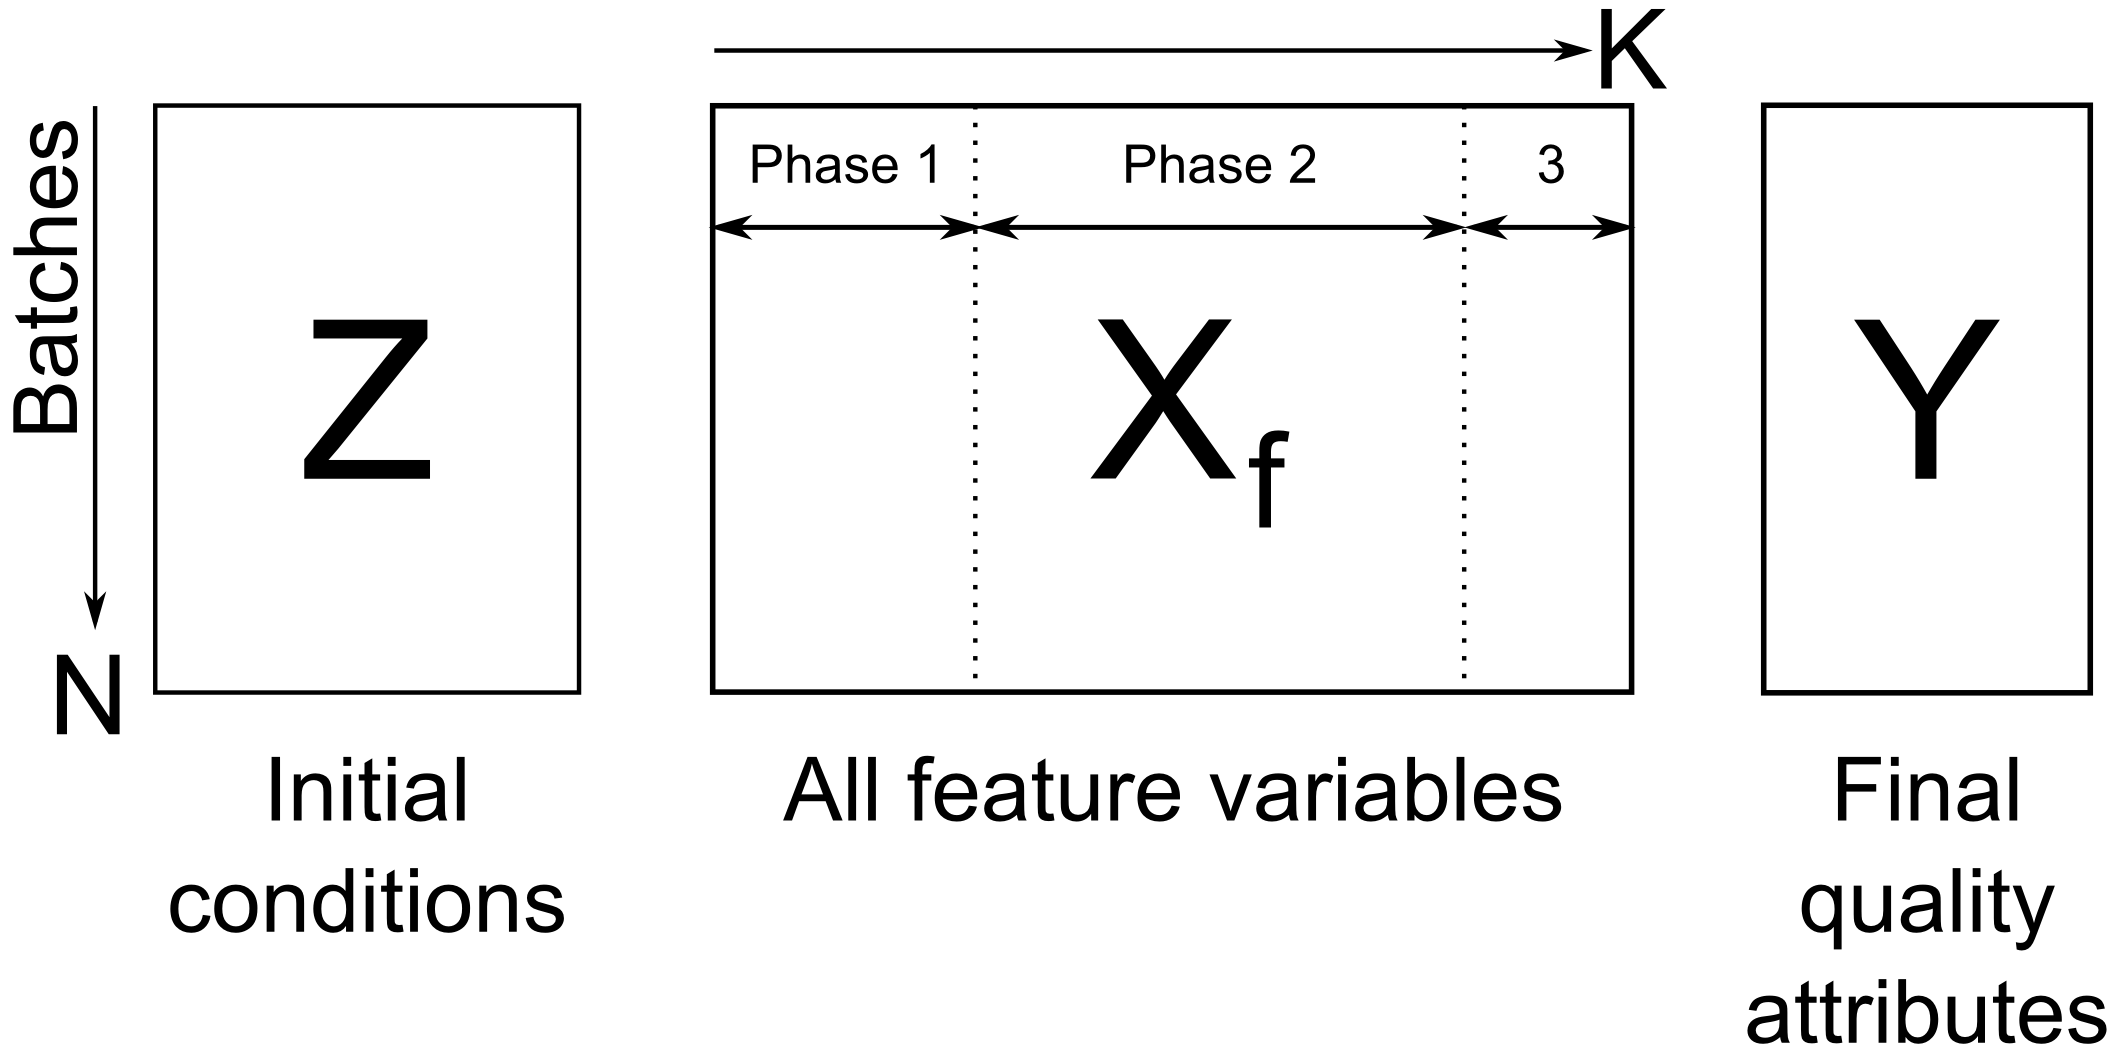
\includegraphics[width=0.95\textwidth]{images/data-after-feature-extraction.png}
\end{center}
\end{frame}

\begin{frame}\frametitle{Which features to extract}

\begin{itemize}
	\item	Extract {\color{myGreen}{\emph{within each phase}}} or within {\color{myGreen}{\emph{specified windows}}}. 
	
	\item	Extract for one, some, or \textbf{all} tags:
\end{itemize}\pause

\begin{itemize}
	\item	average value \hfill {\color{myOrange} $\leftarrow$ easiest, most useful feature}
	\item 	median value
	\item	integrated area under a tag (often makes engineering sense)
	\item	standard deviation, (useful if tag should be constant)
	\item	slope of curve\pause
	\item	energy or mass balance calculation over a phase
	 		\begin{itemize}
	 			\item	e.g. heat released by a reaction should be taken up by the cooling water
	 			\item	an imbalance can point out a problematic batch
	 		\end{itemize} \pause
	\item	value of a trajectory at start/end of phase
	\item	total time for a phase to complete (goes into \( \mathbf{Z} \))
\end{itemize}
\end{frame}

\begin{frame}\frametitle{How to use feature-based models}

\begin{itemize}
	\item	Many features extracted: often \( \sim \) 80 to 100 columns; many are not useful
	
	\item	Used in an ordinary PCA or PLS.  All the usual tools apply:
	
			\begin{itemize}
				\item	VIP: finds most import variables for explaining FQAs \( (\mathbf{Y}) \)
				
				\item	loadings and weights: used to interpret any clusters in the scores
				
				\item	use \( R^2 \) per variable and small weights to decide which on less-useful features to eliminate
			\end{itemize}\pause
	
	\item	Learn about the batch: {\small e.g.: variability in cooling water temperature related to poor FQA}
	
	\item	Troubleshooting an unusual batch 

	\item	By extension, use troubleshooting information to improve future batches \pause
	
	\item	Can be used for monitoring: we'll come back to this
\end{itemize}
\end{frame}

\begin{frame}\frametitle{Disadvantages of feature-based models}

\begin{itemize}
	\item	Smoothly varying trajectories within a phase
	
			\begin{itemize}
				\item	no distinct features and hard to quantify
			\end{itemize}

\end{itemize}

\begin{center}
	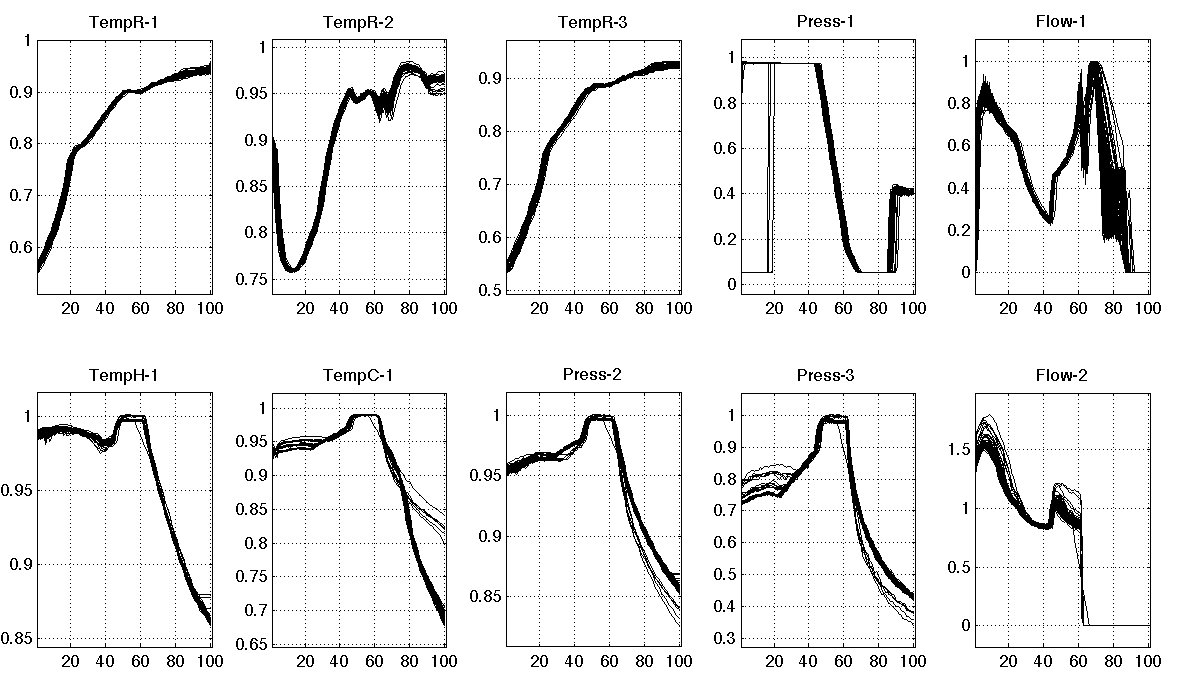
\includegraphics[width=\textwidth]{images/smooth-trajectories-unsuitable-for-features.png}
\end{center}

\end{frame}

\begin{frame}\frametitle{Disadvantages of feature-based models}

\begin{itemize}
	\item	Features to choose depend on engineer's prior knowledge
	
	\item	Subtle defects and broken correlations between variables 
	
			\begin{itemize}
				\item	hard/impossible to detect and quantify
			\end{itemize}

	\item	Feature value may not exist in an abnormal batch: so it's missed

\end{itemize}

\begin{center}
	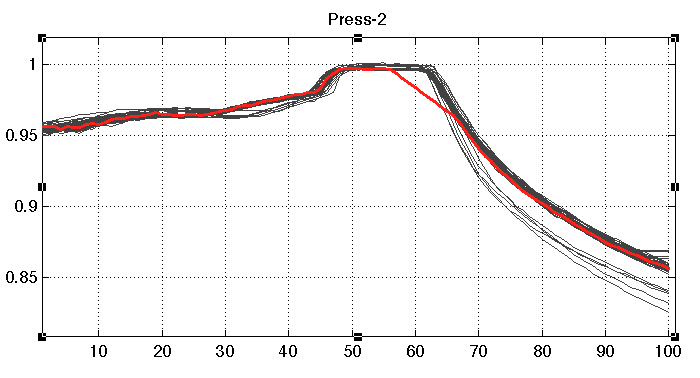
\includegraphics[width=0.9\textwidth]{images/features-subtle-problems-can-go-undetected.png}
\end{center}

\end{frame}

\begin{frame}\frametitle{Class example: using feature-based models}

	\begin{itemize}
		
		\item	Feature example for this batch process works well
		
				\begin{itemize}
				
					\item	4 distinct phases with ``sharp'' trajectories
				
				\end{itemize}

	\end{itemize}

	\begin{center}
		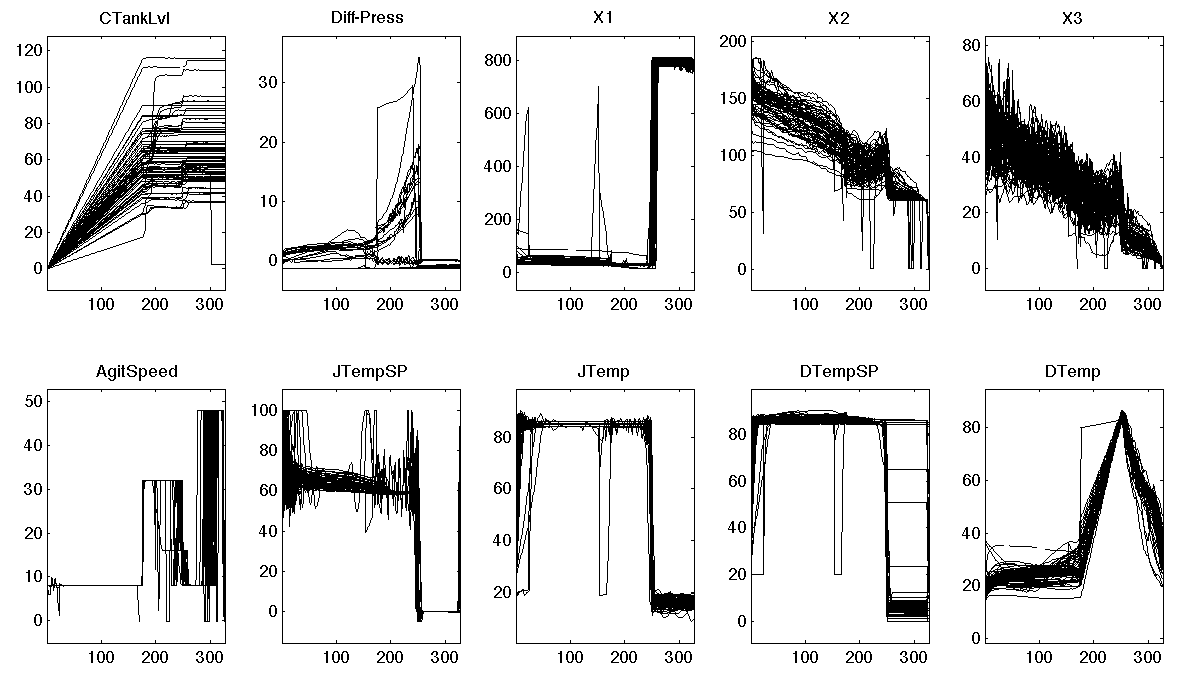
\includegraphics[width=\textwidth]{images/fmc/fmc-raw-trajectories.png}
	\end{center}

\end{frame}

\begin{frame}\frametitle{Class example: using feature-based models}

	\begin{itemize}
	
		\item	Features already extracted for you in the data file
	
	\end{itemize}

	\begin{center}
		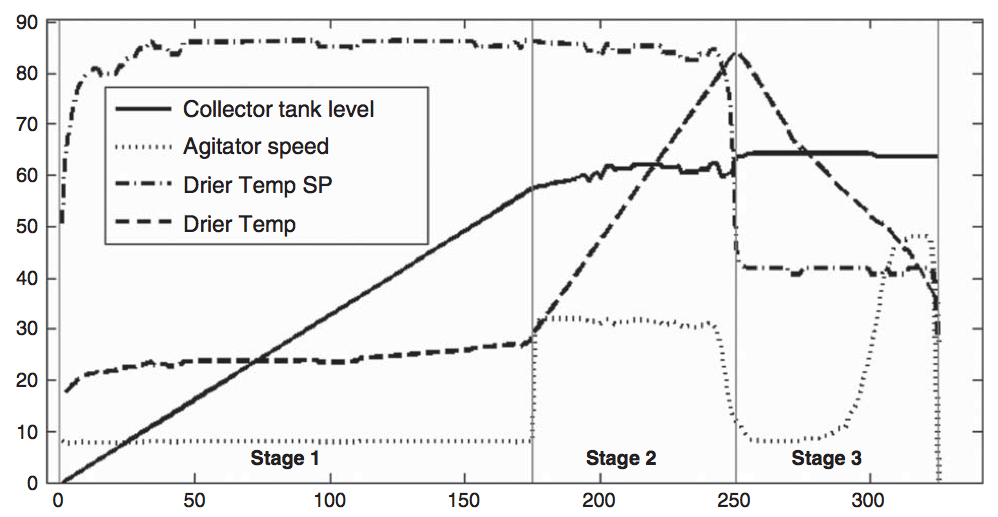
\includegraphics[width=\textwidth]{images/fmc/fmc-phases-4-trajectories.png}
	\end{center}
	
\end{frame}

\begin{frame}\frametitle{Class example: using feature-based models}

	\begin{itemize}
	
		\item	Features already extracted for you in the data file
	
	\end{itemize}

	\begin{center}
		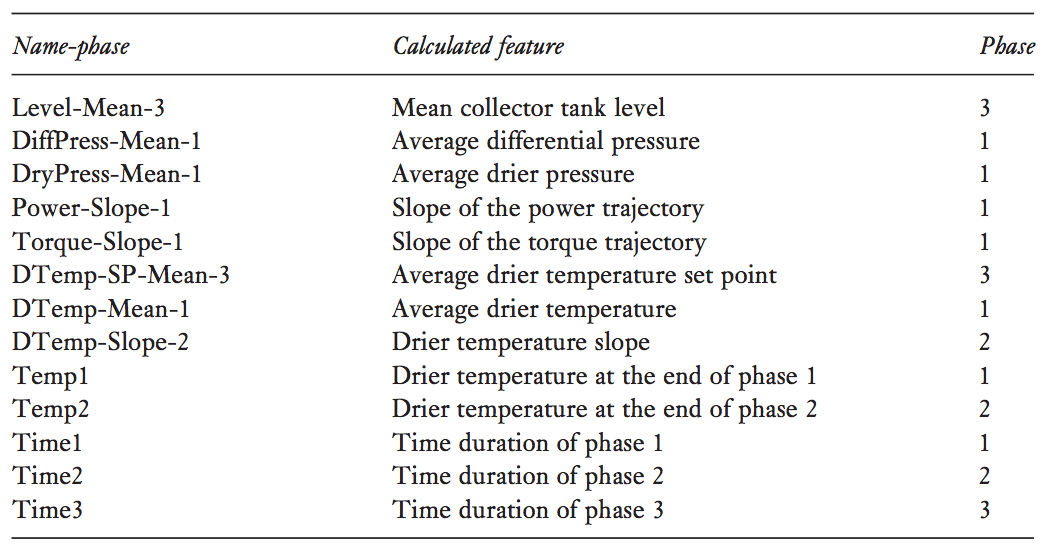
\includegraphics[width=\textwidth]{images/fmc/fmc-features-extracted.png}
	\end{center}

\end{frame}

\begin{frame}\frametitle{Class example: model structure for features}

	\begin{itemize}
		\item	Features compiled into a multiblock PLS model
		
				\begin{itemize}
					\item	\( \mathbf{Z} \): recipe information and composition of material charged (11 variables)
					
					\item	\( \mathbf{X} \): the 13 extracted features
					
					\item	\( \mathbf{Y} \): 8 final quality variables
				\end{itemize}
	\end{itemize}
	
	\begin{center}
		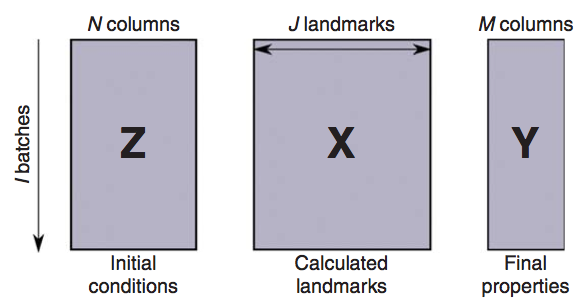
\includegraphics[width=\textwidth]{images/fmc/fmc-features-multiblock.png}
	\end{center}
\end{frame}

\begin{frame}\frametitle{Class example: model results}
	
	\begin{itemize}
		\item	Score plot shows good clear separation between off-spec batches (red circles) and good product (black squares)
	\end{itemize}

	\begin{center}
		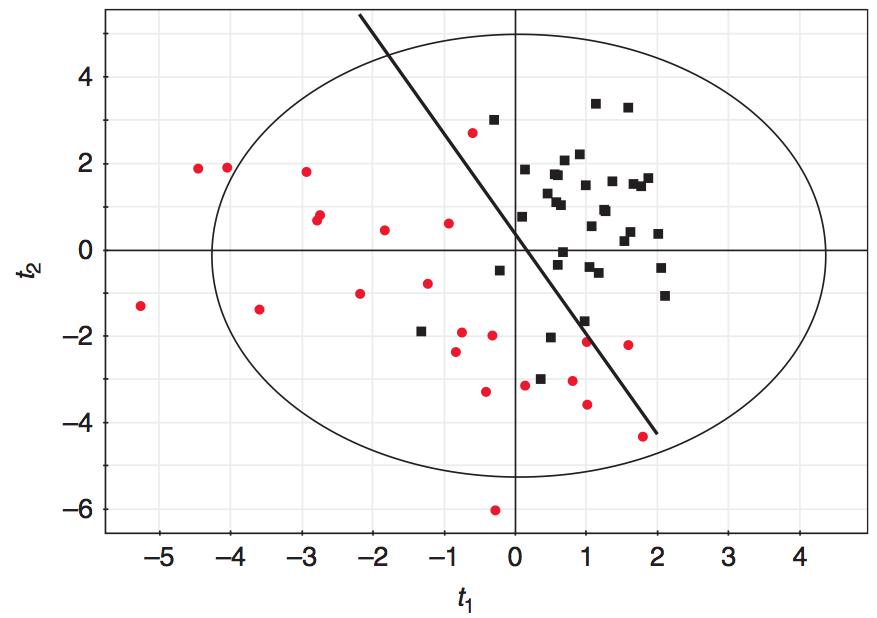
\includegraphics[width=0.9\textwidth]{images/fmc/fmc-score-plot-features.png}
	\end{center}
\end{frame}

\begin{frame}\frametitle{Class example: model results}
	
	\begin{itemize}
		\item	Loading plot for \( \mathbf{Z} \) and \( \mathbf{X} \) blocks
	\end{itemize}
	
	\begin{center}
		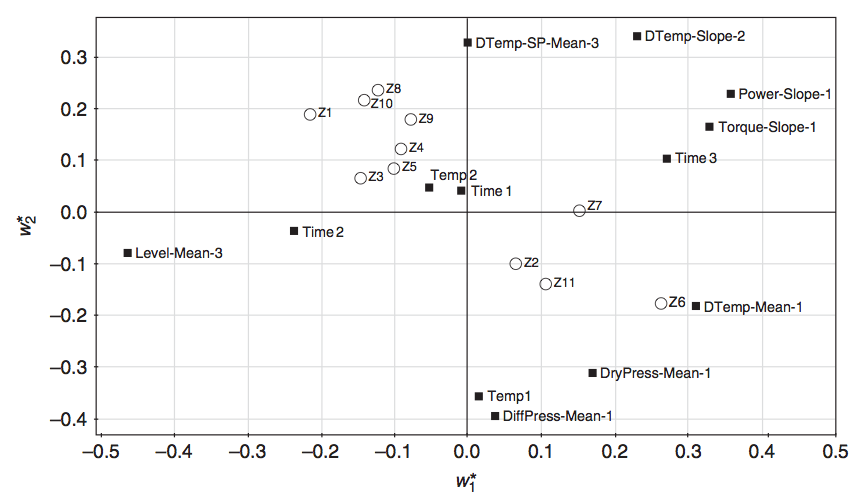
\includegraphics[width=\textwidth]{images/fmc/fmc-features-loading-plot.png}
	\end{center}
	
\end{frame}

\begin{frame}\frametitle{Class example: model results}
	
	\begin{itemize}
		\item	VIP for \( \mathbf{Z} \) and \( \mathbf{X} \) blocks. Agrees with loadings.
	\end{itemize}
	
	\begin{center}
		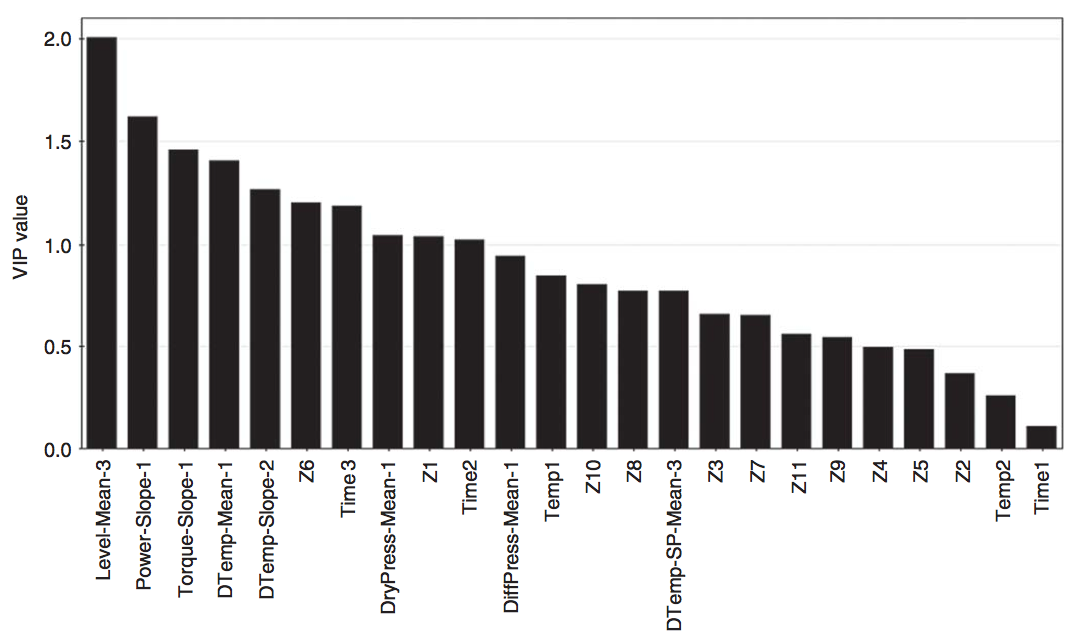
\includegraphics[width=\textwidth]{images/fmc/fmc-VIP-values-features.png}
	\end{center}
\end{frame}

\begin{frame}\frametitle{Class example: what was learned?}
	
	To get good quality batches: operate at high \( t_1 \) and high \( t_2 \).  From loadings plot:
	
	\begin{itemize}
		\item	he plot shows that high rates of increase (slopes) of power, torque, and temperature in phase 1, as well as low solvent level in the collector tank in phase 3 (equivalent to low initial solvent in the wet cake) all relate to a good batch outcome
		% High t1: lower JTempSP slope:  But, JtempSlope is between -0.15 and -0.05, so a lower JTempSlope implies 
		% operation toward -0.15, ie temperature decreases more rapidly for the good batches. This might appear conflicting with the w*1 line plot, which shows that higher values of temperature SP lead to better batches.  How can a batch with a steeper decreasing slope have high value of temperature SP?  Well, the key insight is that temperature SP is always going to END at the same temperature value at the end of phase 2.  Having a steeper, more negative slope, implies that the batch must start at a higher temperature earlier in the batch.  This agrees exactly with the w*1 line plot.
	\end{itemize}
	
	Can be confirmed by looking at what trajectories for some good quality batches.
	
	\todo{Plot good quality batches}
	
\end{frame}


% 
% %-------------------------------------------------
\section{Batch analysis via direct PCA and PLS}
%-------------------------------------------------

\begin{frame}\frametitle{Batch systems: simple definition}

\begin{exampleblock}{Simplest definition}
\centering{\large{\textbf{A batch system}: group of the \alert{\emph{same variables}}, gathered over a period of \alert{\emph{time}}}}
\end{exampleblock}
	
\begin{center}
	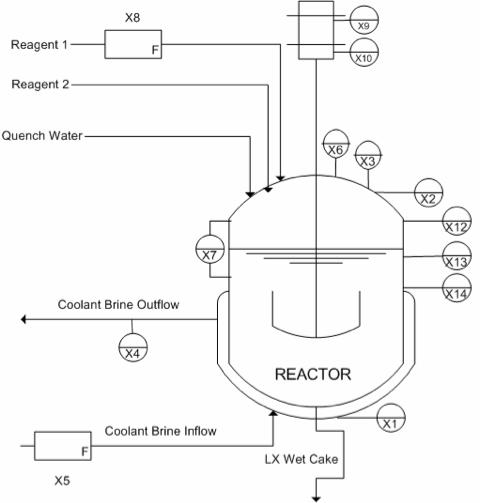
\includegraphics[width=6cm]{images/batch-system.png}	
\end{center}

\end{frame}	

\begin{frame}\frametitle{Batch systems: changing relationship}

	\textbf{Batch system}: group of the \emph{same variables}, gathered over a period of \emph{time}.  Why not just use ordinary PCA or PLS:

	\begin{center}
		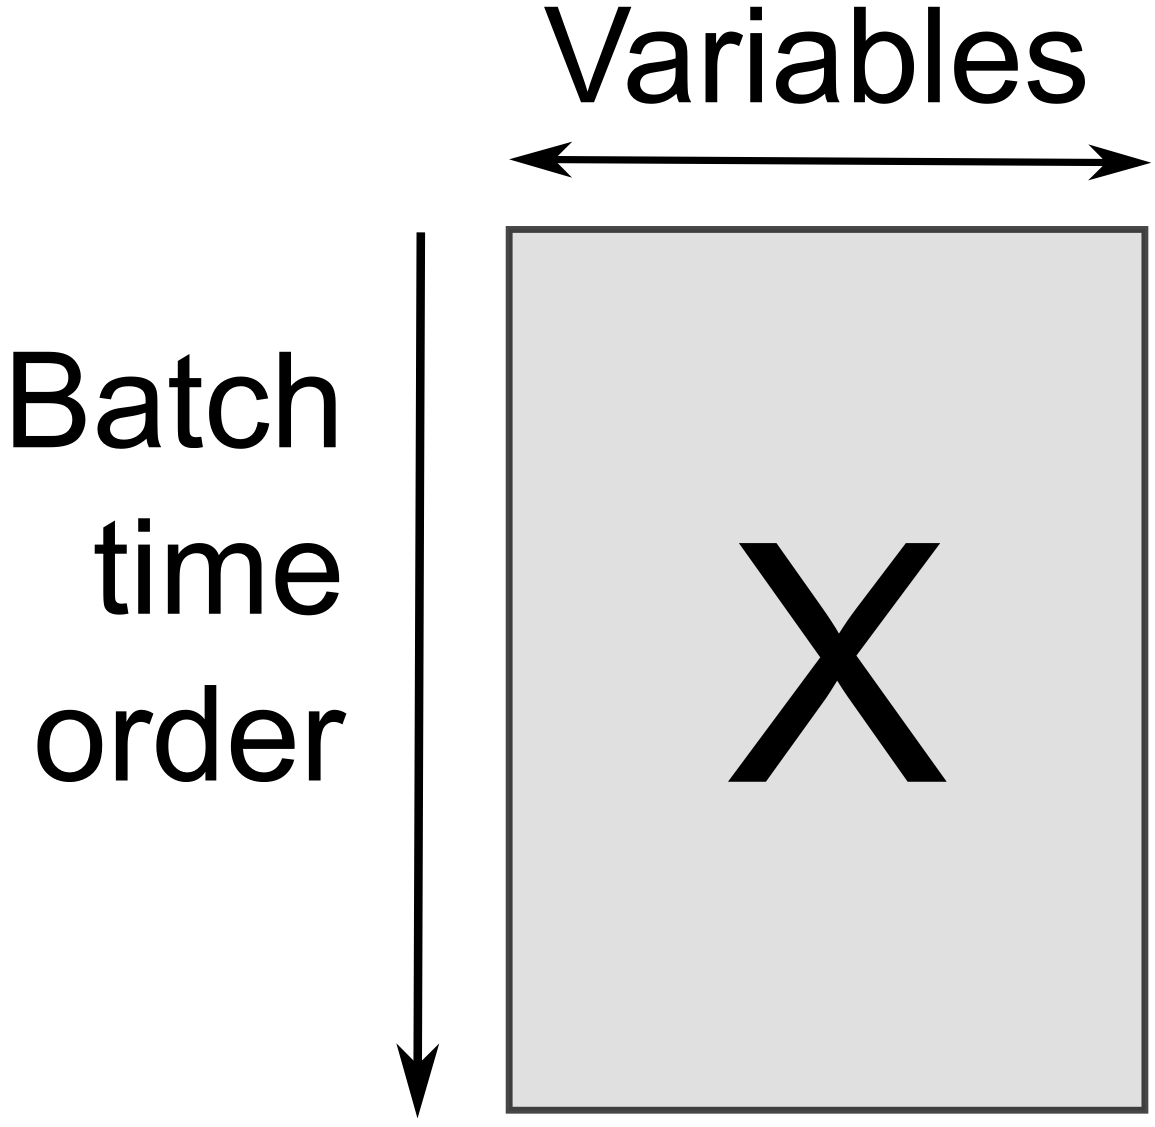
\includegraphics[width=2.4cm]{images/batch-illustrate-unusual-unfolding.png}
	\end{center}


	\begin{itemize}
		\item 	PCA is invariant to row order: 
		\begin{itemize}			
			\item	can shuffle rows, still get same model
			\item 	explain how rows are related to each other
			\item 	each row is assumed independent of the others
			\item 	summarize relationship between variables (columns)
		\end{itemize}
	\end{itemize}

	\begin{exampleblock}{Key issue}
	In \textbf{batch systems}: relationship between variables \alert{changes during the batch}
	\end{exampleblock}
\end{frame}

\begin{frame}\frametitle{Batch systems: changing relationship}

\begin{enumerate}
	\item Relationship between variables change within a batch 
			\begin{itemize}
				\item 	Entry and exit temperatures in a batch dryer correlate (move together) at the end of the batch. 
				\item 	At start of the batch there is little relationship: heat used to evaporate moisture	
			\end{itemize}\pause

	
	\item Past history of a batch affects future behaviour (``integrating system'')
	
			\begin{itemize}
				\item 	Unfold batch data as shown above: cannot capture that ``past effect'' on future rows.  Why?
				\item  	Recall: each row is independent in PCA and PLS
			\end{itemize}

\end{enumerate}
\end{frame}

\begin{frame}\frametitle{Batch systems: changing relationship}
\begin{enumerate}
	\setcounter{enumi}{2}
	\item 	Predictive modelling is harder by unfolding this way

			\begin{center}
				\includegraphics[width=3.5cm]{images/batch-illustrate-unusual-unfolding-with-Y.png}
			\end{center}
			
		
			\begin{itemize}
				\item 	What do we use as the \( \mathbf{Y} \) matrix in this case? {\scriptsize We don't have  \( \mathbf{Y} \) values at each time step.}
				\item 	Many elaborate schemes proposed in literature.			
			\end{itemize}
		
	\item 	Simple solution: arrange data so that each batch is within a row
	
			\begin{itemize}
				\item 	There are some issues with this  (alignment, real-time monitoring)
				\item 	In general, these issues can be addressed effectively
			\end{itemize}
\end{enumerate}
\end{frame}

\begin{frame}\frametitle{Analysis and learning from batch data}

	\begin{exampleblock}{Approach}
	Unfold the aligned batch data row wise, one batch per row, and use PCA and PLS directly.
	\end{exampleblock}

	\begin{center}
		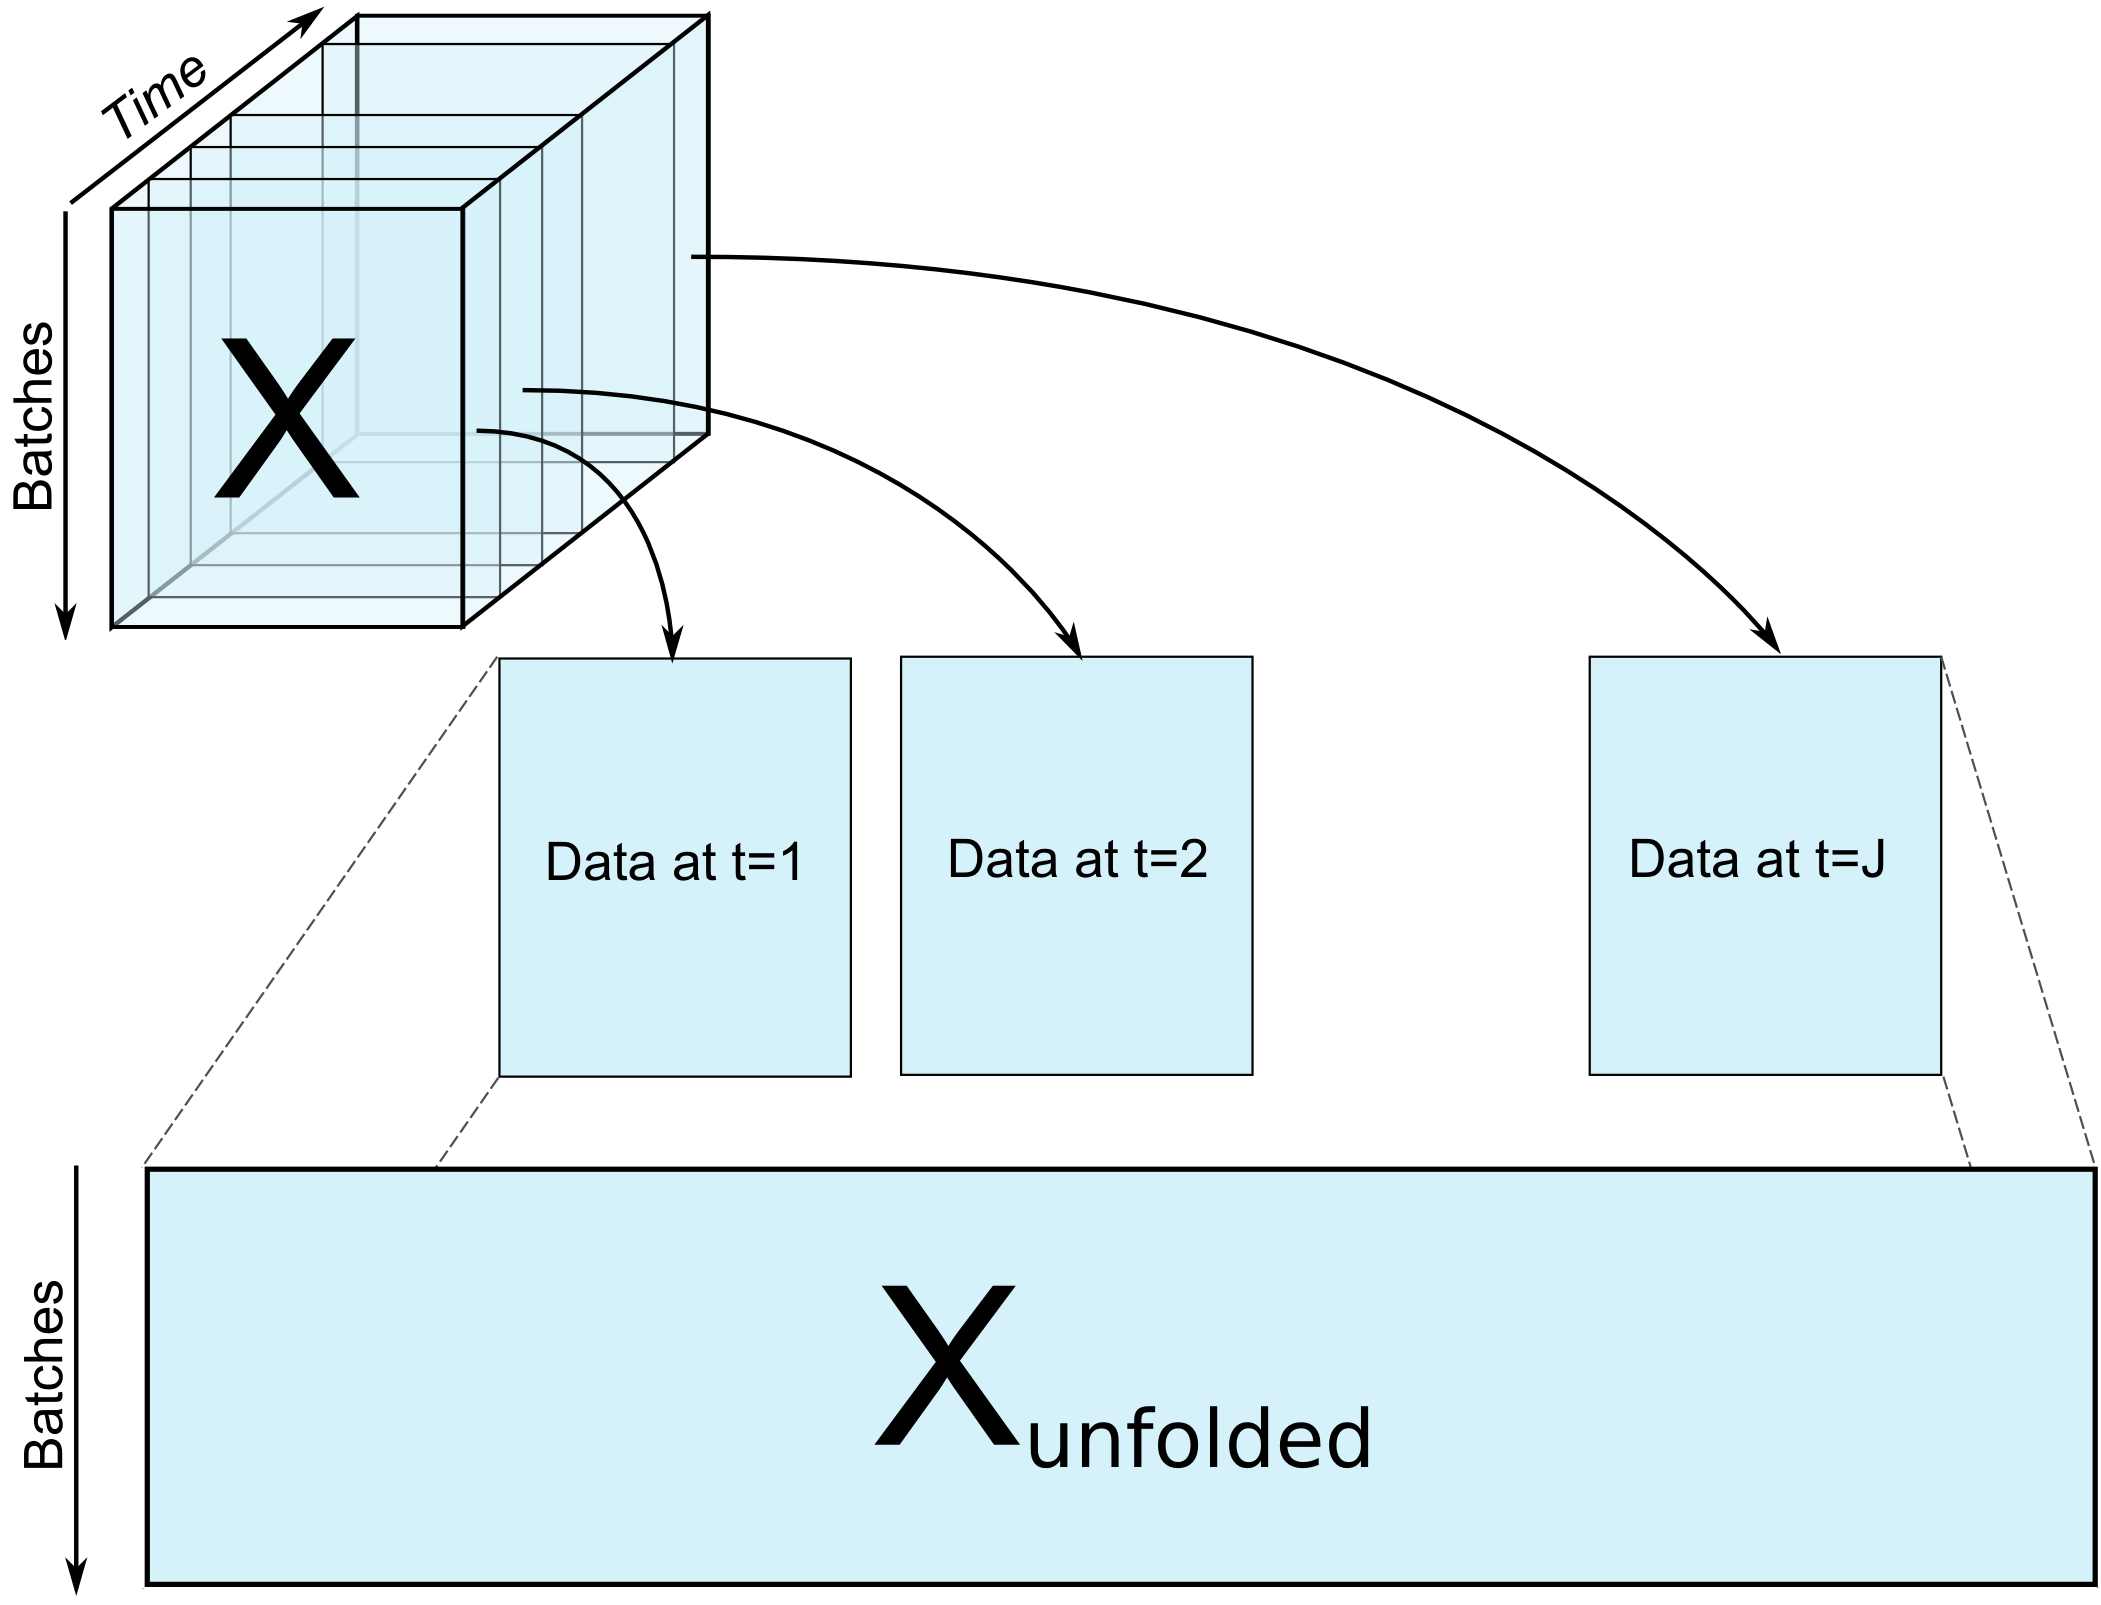
\includegraphics[width=8cm]{images/batch-data-unfolding-X-only.png}	
	\end{center}
\end{frame}	


% 
% %!TEX root = batch-course.tex

\begin{frame}\frametitle{Batch PCA example: SBR}
	
	\begin{itemize}
		\item	Simulated data from \emph{large} mechanistic model for styrene butadiene rubber
		
		\item	Good to start learning from this case study
		
		\item	Simulated to contain ``normal operating conditions''
		
				\begin{itemize}
					\item	2 main problematic batches
					
					\item	same fault, but starting at different times
				\end{itemize}
	\end{itemize}
	
\end{frame}

\defverbatim[colored]\loaddata{%
\begin{lstlisting}[basicstyle=\tt\scriptsize\color{myOrange},frame=none,language=C++,linewidth=.9\textwidth]

data = load('datasets/SBR.mat');   % X is in a  10600 x 9 matrix
Y_data = data.Y;
   
% Specify the data dimensions
nBatches = 53;
nTags = 6;
nSamples = 200;  % not required
tagNames = {'Reactor temperature', 'Cooling water temp', ...
            'Reactor jacket temperature', 'Latex density', ...
            'Conversion', 'Energy released'};
        
% Create a batch block first: tell it how many batches 
% there are in the aligned data
% Ignore tags 1, 2, 3 (noisy and uninformative)

batchX = block(data.X(:, 4:9), 'X', 'batch', ...
               'tagNames', tagNames, 'nBatches', nBatches);
\end{lstlisting}}

\begin{frame}[fragile,containsverbatim]\frametitle{SBR: load the data}
	\loaddata
\end{frame}

\begin{frame}\frametitle{SBR: raw data}
	
	\begin{itemize}
		\item	Batches: \( N = 53 \); Tags: \( K = 6 \); Time steps: \( J = 200 \)
		
	\end{itemize}
	
	\begin{center}
		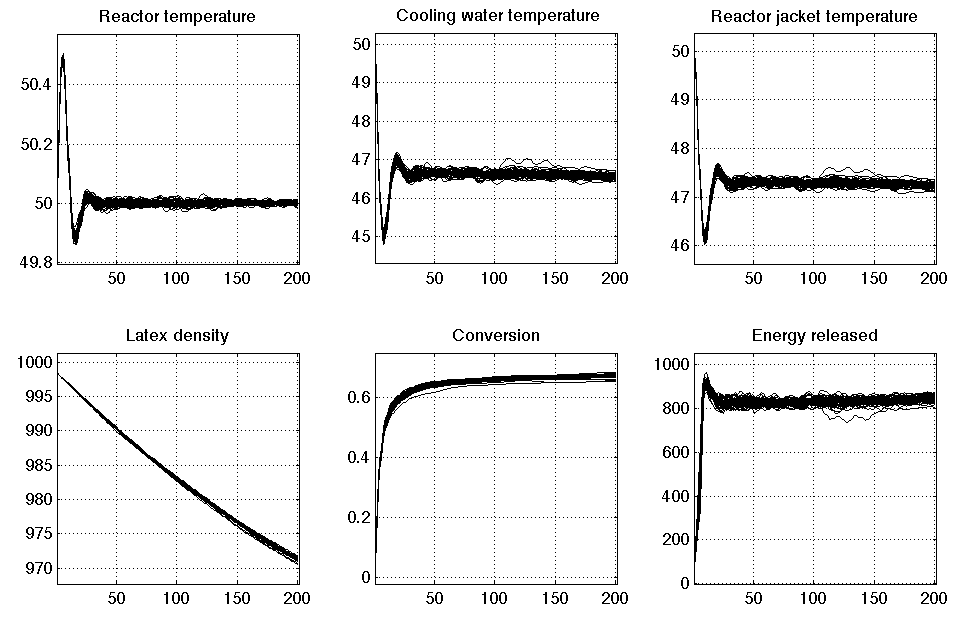
\includegraphics[width=\textwidth]{images/sbr/SBR-raw-data-trajectories.png}
	\end{center}
	{\color{myOrange}{\texttt{plot(batchX, 'raw', 2, 3)}}}
\end{frame}

\begin{frame}\frametitle{SBR: build model}
	
	\begin{itemize}
		\item	Start with 2 to 3 components: \emph{just to see what's going on}
		
		\item	{\color{myOrange}{\texttt{batch\_PCA = lvm(\{'X', batchX\}, 2)}}}
		
		\item	\( R^2_1 = 24.5\% \) and \( R^2_2 = 13.3\% \)
		
		\item	Next: scores, loadings, SPE, \( T^2 \) (all the usual PCA tools)
		
	\end{itemize}

\end{frame}

\begin{frame}\frametitle{SBR: scores and \( T^2 \)}
	
	\begin{center}
		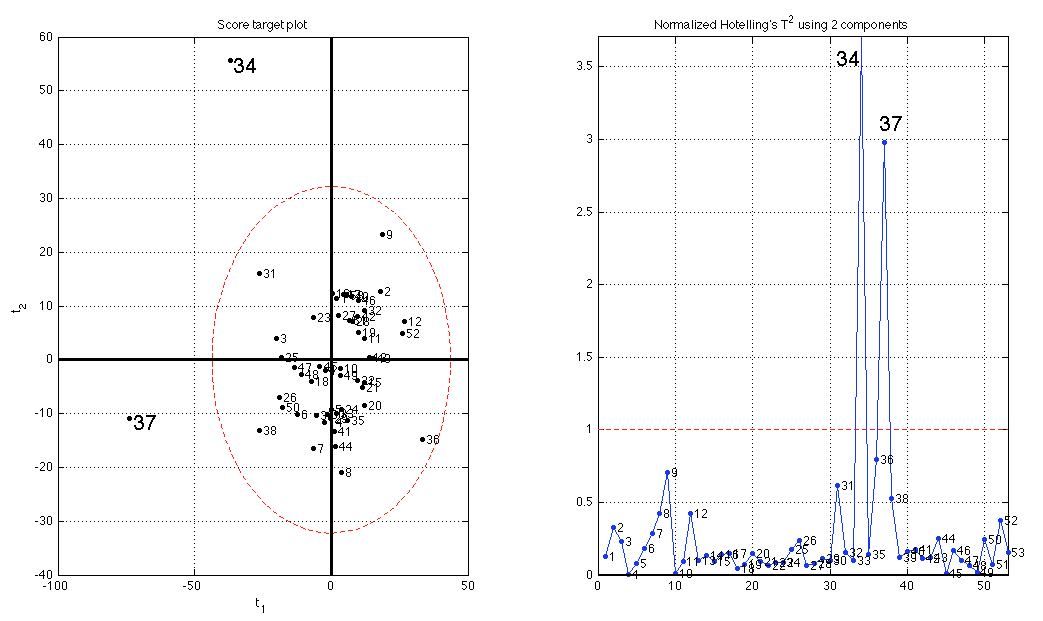
\includegraphics[width=0.8\textwidth]{images/sbr/SBR-scores-and-T2.png}
	\end{center}

	\begin{itemize}
		\item	{\color{myOrange}{\texttt{plot(batch\_PCA, 'scores')}}}
		
		\item	Batch 34 and 37 had differences in their progress from bulk of other batches\pause
		
		\item	These were in fact the unsuccessful batches!  This shows promise.
	\end{itemize}

\end{frame}

\begin{frame}\frametitle{SBR: check SPE}
	
	\begin{center}
		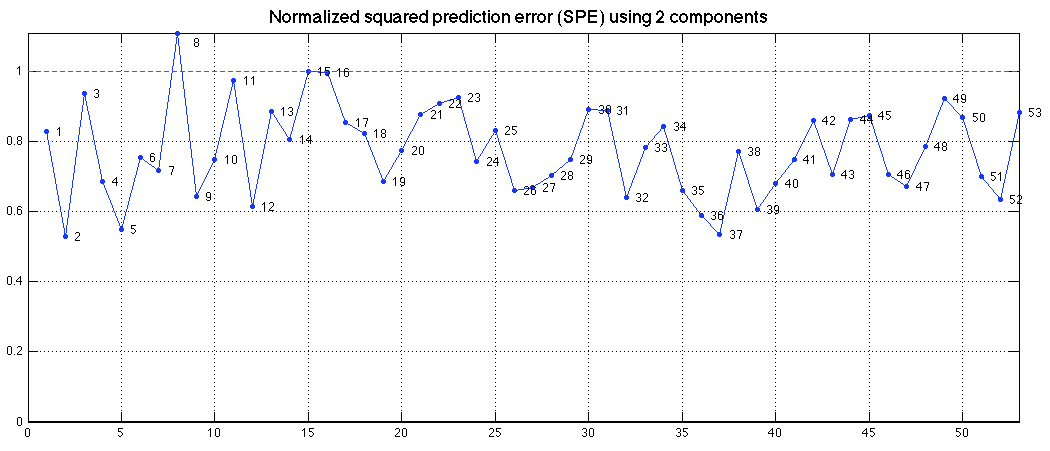
\includegraphics[width=0.8\textwidth]{images/sbr/SBR-SPE-plot-per-batch.png}
	\end{center}

	\begin{itemize}
		\item	{\color{myOrange}{\texttt{plot(batch\_PCA, 'spe')}}}
		
		\item	No problems picked up.  This is the overall SPE, using data from the \emph{entire} batch.
	\end{itemize}

\end{frame}

\begin{frame}\frametitle{SBR: understand \( R^2 \) breakdown}
	
	\begin{center}
		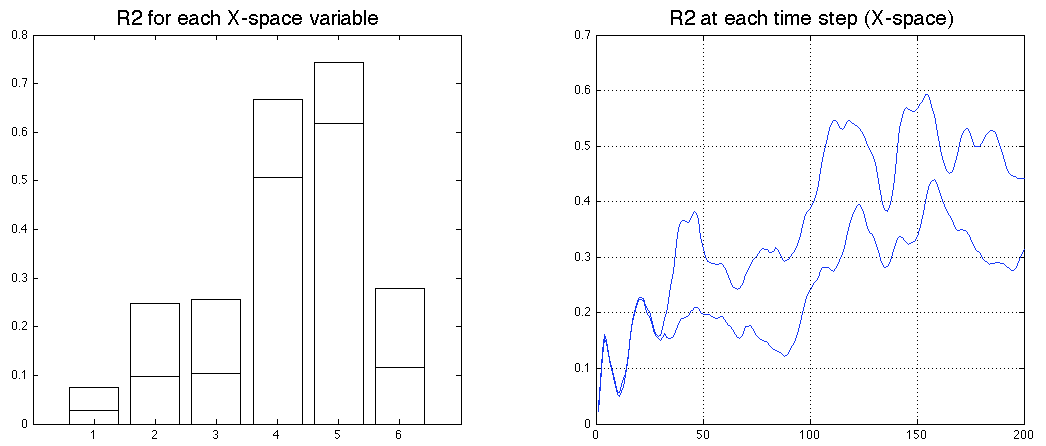
\includegraphics[width=0.8\textwidth]{images/sbr/SBR-R2-over-batch.png}
	\end{center}

	\begin{itemize}
		\item	{\color{myOrange}{\texttt{plot(batch\_PCA, 'R2')}}}
		
		\item	LV1: Tags 4 (latex density) and 5 (conversion) dominate
		
		\item	LV2: explains tags 2, 3, 4, 5, 6 by about 15\% each
		
		\item	LV1: explains everything from \( t = 0 \)  to \( t = 30 \)
		
		\item	\( R^2 \) is low at start because all batches are similar initially
		
				\begin{itemize}
					\item	after centering and scaling there is just noise at the start.
				\end{itemize}
	\end{itemize}

\end{frame}

\begin{frame}\frametitle{SBR: loadings}
	
	\begin{center}
		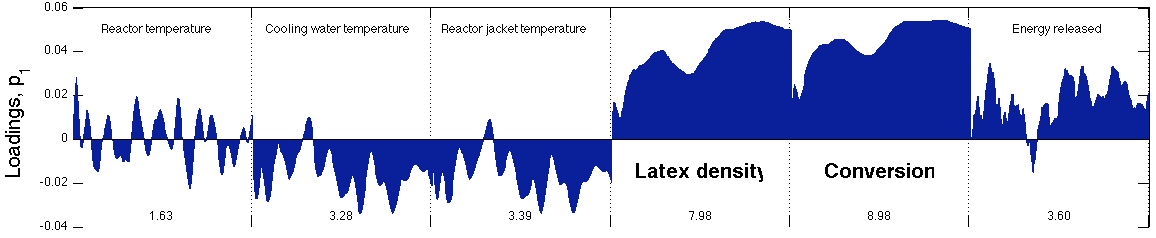
\includegraphics[width=\textwidth]{images/sbr/SBR-loadings-p1.png}
	\end{center}
	\begin{center}
		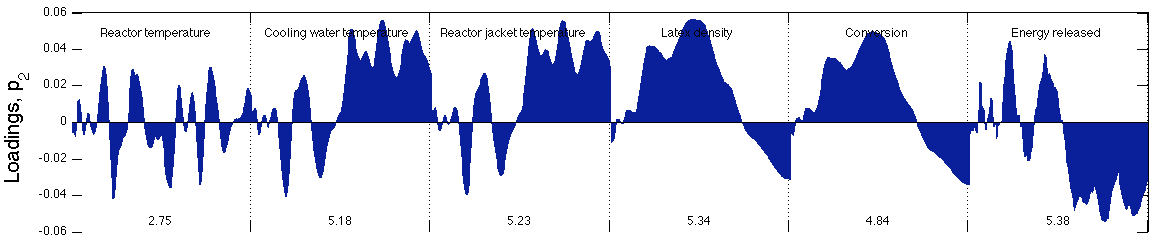
\includegraphics[width=\textwidth]{images/sbr/SBR-loadings-p2.png}
	\end{center}
	
	\begin{itemize}
		\item	Batch 37 [low \( t_1 \)]: below average latex density and conversion throughout the batch
		
		\item	Batch 34:[high \( t_2 \)]: above average cooling water temp, jacket temp, and below avg energy released in last half
		
	\end{itemize}
\end{frame}
 
\begin{frame}\frametitle{SBR: scores \emph{over time} for batch 37}
	
	\begin{center}
		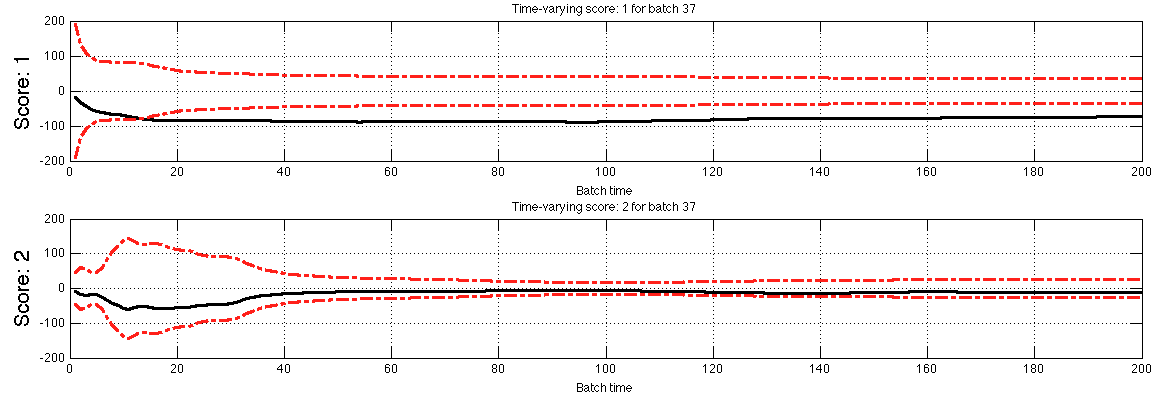
\includegraphics[width=\textwidth]{images/sbr/SBR-time-evolving-scores.png}
	\end{center}
	
	\begin{itemize}
		\item	Don't just have a \( t \)-score at the end, also get the score as batch progresses
		
		\item	Highlights \emph{when} the problem occurred: right at the start
		
				\begin{itemize}
					\item	Was due to an impurity in the feed: consumed reactant and lowers latex density and conversion
				\end{itemize}
	\end{itemize}
	
	{\color{myOrange}{\texttt{plot(batch\_PCA, 'scores', \{'batch', 37\})}}}
\end{frame}

\begin{frame}\frametitle{SBR: contribution plot for batch 37}
	
	\begin{center}
		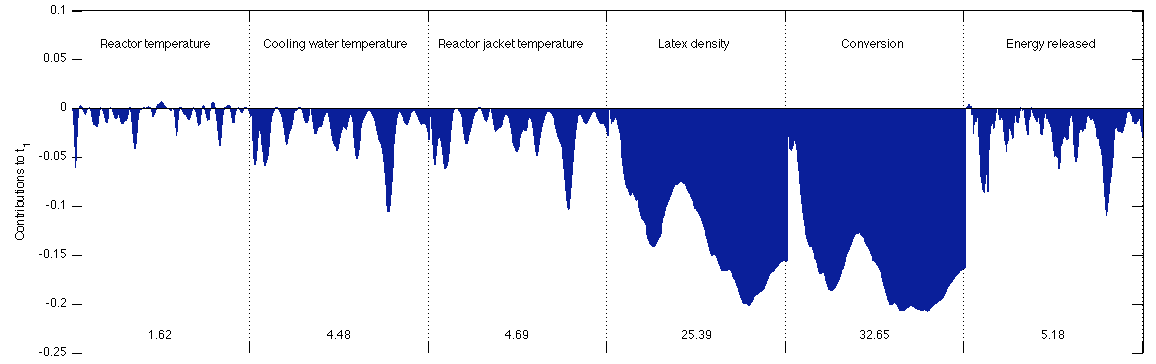
\includegraphics[width=\textwidth]{images/sbr/SBR-contributions-to-batch-37.png}
	\end{center}
	
	\begin{itemize}
		\item	Contributions highest for the latex density and conversion, as expected.
		
				\begin{itemize}
					\item	{\color{myOrange}{\texttt{  contrib\_37 = contrib(batch\_PCA, 37)  }}}
					
					\item	{\color{myOrange}{\texttt{  plot(contrib\_37, 'scores', 1)		  }}}
				\end{itemize}
	\end{itemize}
\end{frame}

\begin{frame}\frametitle{SBR: raw data for batch 37 (to confirm)}
	
	\begin{center}
		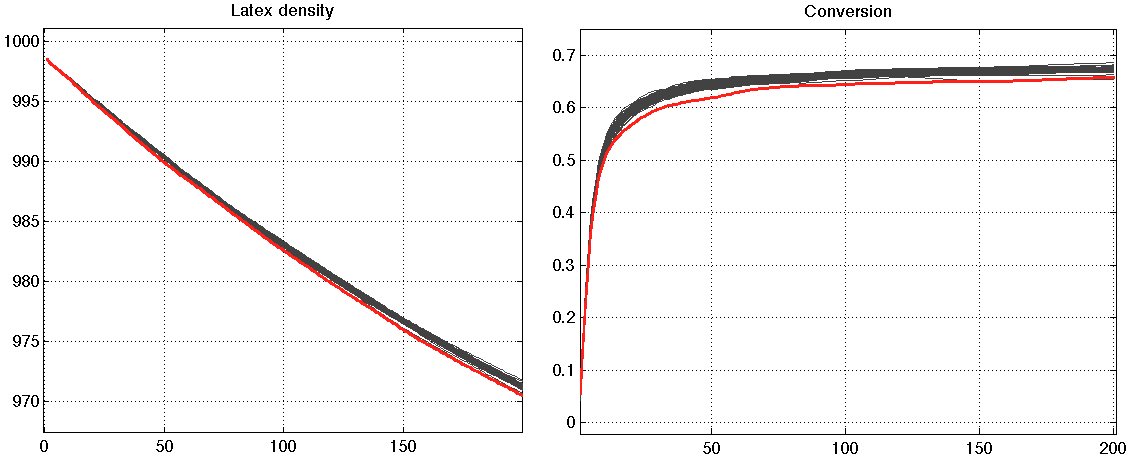
\includegraphics[width=\textwidth]{images/sbr/SBR-raw-data-batch-37-highlighted.png}
	\end{center}
	
	\begin{itemize}
		\item	Confirmed our interpretation with the raw data
				
				\begin{itemize}
					\item	{\color{myOrange}{\texttt{plot(batch\_PCA.X, 'highlight', 2, 3, 37)		  }}}
					
					\item	uses a \( 2 \times 3 \) layout for the raw tags
				\end{itemize}
	\end{itemize}
\end{frame}

\begin{frame}\frametitle{SBR:  batch 34}
	
	\begin{itemize}		
		\item	Let's investigate this together in the software
		
		\item	Main new learning: SPE trajectories
		
				\begin{itemize}
					\item	SPE values also available during the batch, with limits
					
					\item	{\color{myOrange}{\texttt{plot(batch\_PCA, 'spe', \{'batch', 34\})		  }}}
					
				\end{itemize}
	\end{itemize}
				
	\begin{center}
		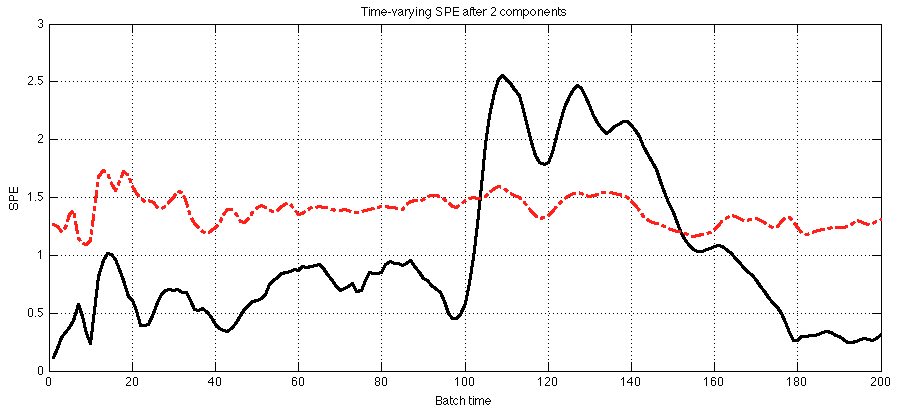
\includegraphics[width=\textwidth]{images/sbr/SBR-time-evolving-SPE-batch-34.png}
	\end{center}
\end{frame}






% 
% %!TEX root = batch-course.tex
\begin{frame}\frametitle{DuPont Nylon example: learning from new data}

	\begin{itemize}
		\item	Industrial data set of \( N = 55 \) batches from Nylon production
		
		\item	Temperature, pressure and flow rate variables: \( K = 10\)  batch tags
		
		\item	Batch duration about 2 hours (\( J=100 \) time intervals)
		
		\item	12 hours before lab values returned: batch-to-batch adjustment not possible
		
		\item	Known problems with batches: 38, 40, 41, 42, 50, 51, 53, 54, 55
	\end{itemize}
	
	
\end{frame}

\begin{frame}\frametitle{DuPont Nylon example: raw data}
	{\color{myGreen}{Note}}: data were scaled for confidentiality
	\begin{center}
		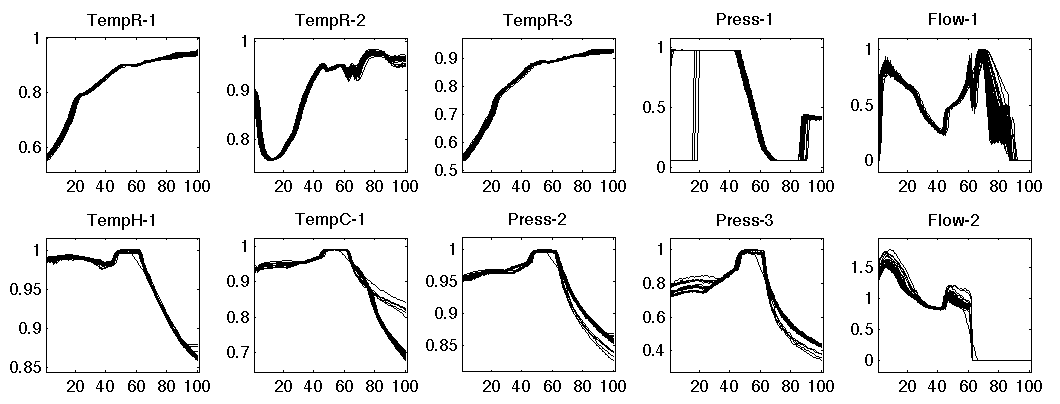
\includegraphics[width=\textwidth]{images/dupont/dupont-raw-data-trajectories.png}
	\end{center}
	
	\vspace{1cm}
	\begin{itemize}
		\item	Can see a few unusual batches: see ``Temp-C1'' and ``Press-1'' tags
		
		\item	Alignment looks pretty good (process is well controlled)
		
		\item	Some periods are noisy: ``Flow-1'' and ``Flow-2''
	\end{itemize}
\end{frame}

\begin{frame}\frametitle{DuPont Nylon example: initial PCA}
	\begin{itemize}

		\item	Just start with 2 components initially
		
				\begin{itemize}					
					\item	no cross-validation, just get a ``feel'' for the data
					\item	\( R^2_X = [38.28\%, 17.58\%]\), or cumulatively: 55.9\%
				\end{itemize}
		
		\item	Score plot: {\color{myOrange}{\texttt{plot(batch\_PCA, 'scores')  }}}
				
				\begin{columns}
					\column{0.8\textwidth}
						\begin{center}
							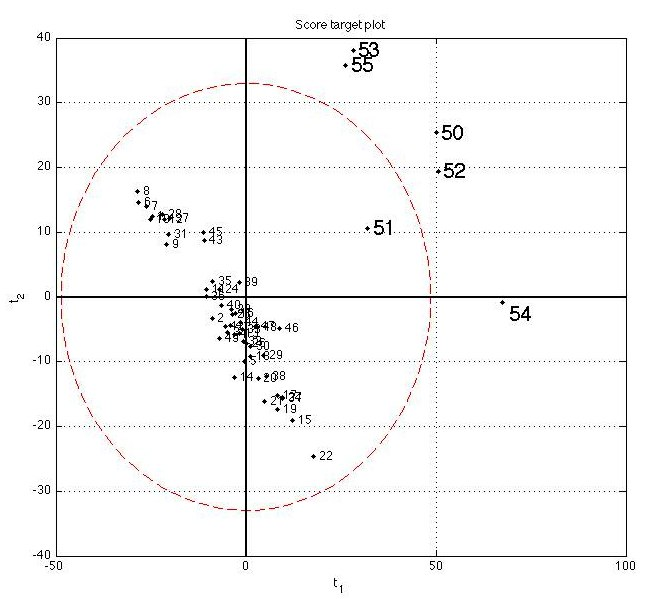
\includegraphics[width=0.8\textwidth]{images/dupont/dupont-raw-score-plot.jpg}
							% batch_PCA = lvm({'X', batch_X}, 2);
							% plot(batch_PCA, 'scores', {'labels'})
						\end{center}
						
					\column{0.4\textwidth}
						\begin{itemize}
							\item	Batches 50 to 55 unusual
							
							\item	Distorted the model		
							
							\item	Before excluding them and rebuilding model, let's first examine them.
						\end{itemize}
				\end{columns}
	\end{itemize}
\end{frame}

\begin{frame}\frametitle{DuPont Nylon example: SPE}
	\begin{itemize}
		\item	SPE plot: {\color{myOrange}{\texttt{plot(batch\_PCA, 'spe')  }}} 
	\end{itemize}
	
	\begin{center}
		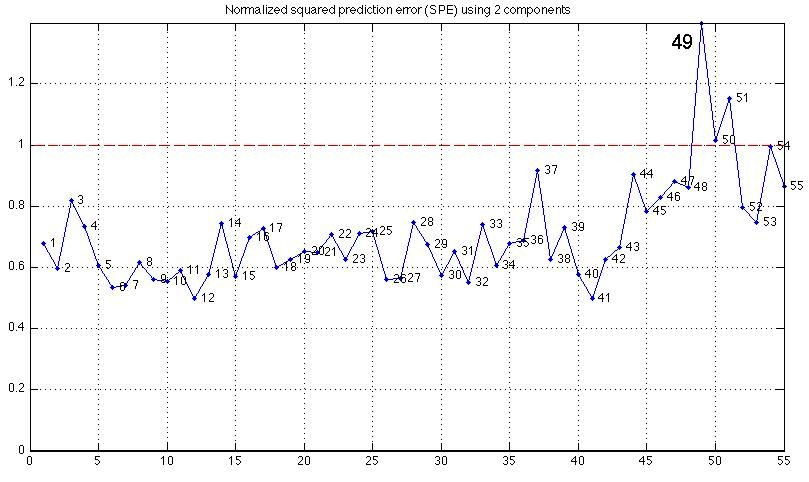
\includegraphics[width=\textwidth]{images/dupont/dupont-raw-SPE.jpg}
	\end{center}
\end{frame}

\begin{frame}\frametitle{DuPont Nylon example: batch 54 (high \( t_1 \) batch)}
	\begin{itemize}
		\item	First plot loadings \( p_1 \) to understand that direction
			
				\begin{itemize}
					\item	{\color{myOrange}{\texttt{plot(batch\_PCA.X, 'loadings', 1)    }}} 
					
					\item	Tags and time periods that are positive in \( p_1 \) will be high in batch 54
					
					\item	The opposite also applies
				\end{itemize}
		
		\item 	Main problems are at the end of the batch:
		
				\begin{itemize}
					\item	Pressures 2 and 3 are below normal
					
					\item	Temp-C1 is above normal
					
				\end{itemize}
		
		\item 	Other problems in Temp-R1 and Temp-R3 at start of the batch
	\end{itemize}
\end{frame}

\begin{frame}\frametitle{DuPont Nylon example: loadings \( p_1 \)}

\begin{center}
	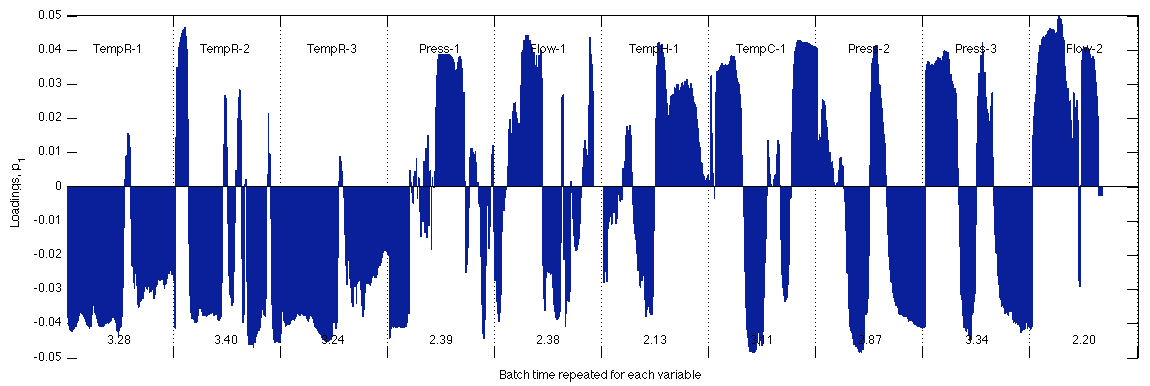
\includegraphics[width=\textwidth]{images/dupont/dupont-loadings-p1.png}
\end{center}

	\begin{itemize}
		\item	Explore other score outliers interactively in class
	\end{itemize}
\end{frame}

\begin{frame}\frametitle{DuPont Nylon example: SPE}

	\begin{itemize}
		\item	Batch 49 shows in the overall SPE 
		
		 		\begin{itemize}
		 			\item	{\color{myOrange}{\texttt{plot(batch\_PCA, 'spe') }}} 
		 		\end{itemize}

		\item 	Also look at the time-varying SPE to see \emph{when} problem occurred: \( t \) = 57 to 67 
		
				\begin{itemize}
					\item	{\color{myOrange}{\texttt{plot(batch\_PCA, 'spe', \{'batch', 49\})  }}} 
				\end{itemize}
		
		\item 	Confirm in contribution plots: tags 6 to 10
	\end{itemize}
	
	\begin{center}
		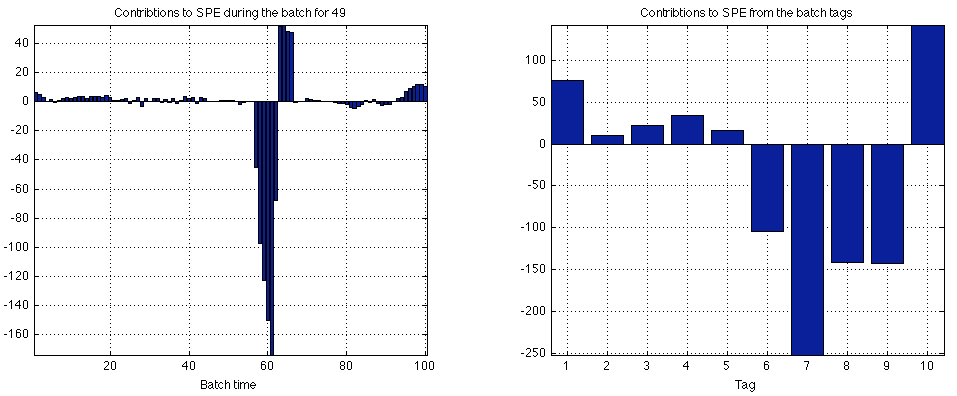
\includegraphics[width=\textwidth]{images/dupont/dupont-batch-49-spe.png}
	\end{center}
\end{frame}

\begin{frame}\frametitle{DuPont Nylon example: Raw data for batch 49}

	\begin{itemize}
		\item	Likely that tag 5 (wrongly) identified as cause
	\end{itemize}
	\begin{center}
		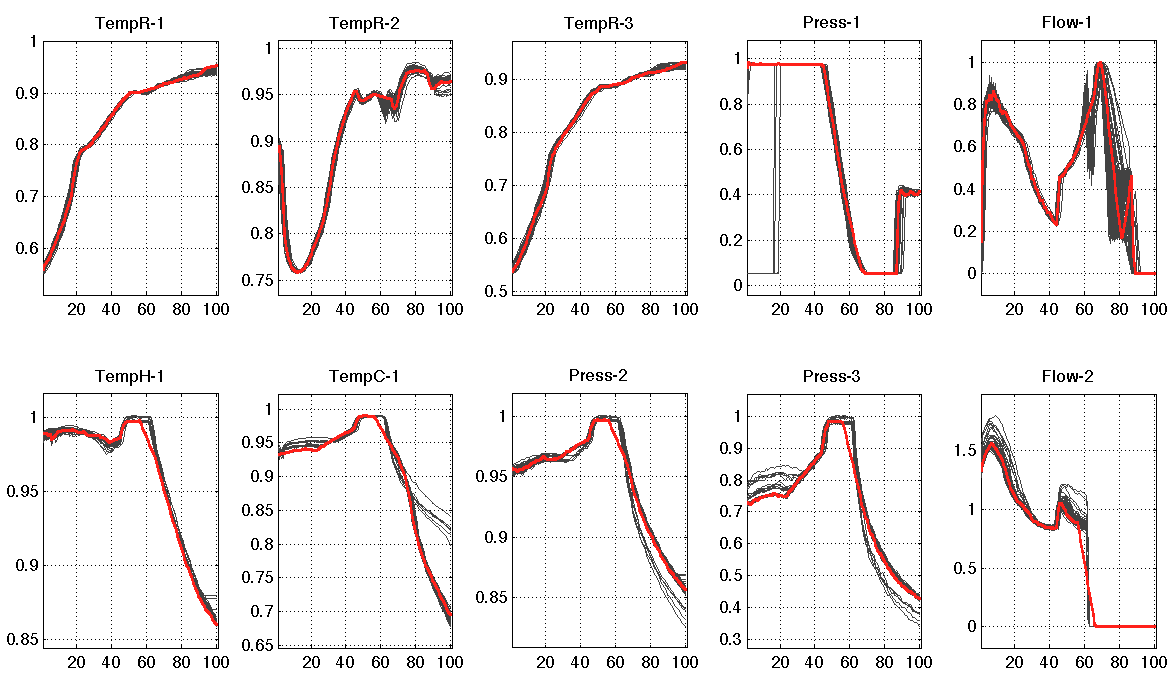
\includegraphics[width=\textwidth]{images/dupont/dupont-highlight-raw-data-batch-49.png}
	\end{center}
	
	\begin{itemize}
		\item	Cause: subtle deviations in heating and cooling system (broken correlation) and pressure system
	\end{itemize}
\end{frame}


% 
% %!TEX root = batch-course.tex
\begin{frame}\frametitle{TODO}
\end{frame}

%!TEX root = batch-course.tex

\begin{frame}\frametitle{Summary: Data understanding and troubleshooting}
	
General procedure to follow:	

	\begin{itemize}
		\item	Plot the trajectories\hfill {\color{myOrange}{\texttt{plot(dataX,'raw', n, m)}}}
	
				\begin{itemize}
					\item	Sometime outlier batches already detectable
				
					\item	Visualize how good your alignment is: do data need extra pretreatment?
				\end{itemize}
			
		\item	Initially include all batches
	
		\item	Build model on all data (usually \( A \) = 2 to 3 components)
		
				\begin{itemize}
					\item	{\color{myOrange}{\texttt{model = lvm({'X', dataX}, A);  }}}
				\end{itemize}
	\end{itemize}
\end{frame}

\begin{frame}\frametitle{Summary: Data understanding and troubleshooting}
	
	Score plots:\hfill {\color{myOrange}{\texttt{plot(model,'scores')}}}

	\begin{itemize}
		\item	Clusters due to seasonal effect?
		
		\item	Different types of abnormalities (faults) will cluster together.
		
		\item	Different product grade clusters?
		
		\item	Raw material suppler change over groupings?
		
		\item	Outliers? Usually we know which batches were bad.  We usually (always?) start to see bad batches in the scores.
		
		\item	Most informative: \( t_1 - t_2 \) and \( t_1 - t_3 \) and \( t_2 - t_3 \)
	\end{itemize}

\end{frame}

\begin{frame}\frametitle{Summary: Data understanding and troubleshooting}
	
SPE plots: \hfill {\color{myOrange}{\texttt{plot(model,'spe')}}}

\begin{itemize}
	\item	There are 2 types:
	
			\begin{itemize}
				\item	overall (available at the end of the batch)
				
				\item	instantaneous (evolving, during the batch)
			\end{itemize}
			
	\item	Contributions to SPE show \emph{which variables} had a changed relationship
	
	\item	and at \emph{what time} during the batch
	
	\item	Should always be verified in the raw data
\end{itemize}

\end{frame}

\begin{frame}\frametitle{Summary: Data understanding and troubleshooting}
	
\begin{itemize}
	\item	Loadings (PCA) and weights (PLS):  
	
			\begin{itemize}
				
				\item	{\color{myOrange}{\texttt{plot(model.X,'loadings')}}}
				
				\item	shows \emph{which variables} and at \emph{what times} they dominate each latent variable
				
			\end{itemize}


	\item 	\( R^2 \) plots\hfill {\color{myOrange}{\texttt{plot(model,'R2')}}}
		
			\begin{itemize}
				\item	interpreted in combination with loadings plot
				
				\item	common to see one latent variable dominating variance explained in a phase (e.g LV1 for phase 2 and LV1 in phase 3)
				
				\item	noisy tags: show low \( R^2  \) and small loadings in components at all times.  Good candidates for removal if:
				 		
						\begin{itemize}
							\item	never used in any contributions, or to explain outliers
							
							\item	unrelated to explaining quality variables
						\end{itemize}
				
				\item	large loading and high \( R^2 \): very important variable for that component
			\end{itemize}

\end{itemize}

\end{frame}

\begin{frame}\frametitle{Summary: Data understanding and troubleshooting}

Removing observations:	
\begin{itemize}
	\item	Remove observations once contributions fully understood, especially if they distort score space
	
	\item	Can be tedious, but important to learn which batch problems are prevalent
	
	\item	Once removed, only common cause batches left:
	
			\begin{itemize}
				\item	we will use that as reference database for monitoring!
			\end{itemize}

\end{itemize}

\end{frame}

%!TEX root = batch-course.tex
%-------------------------------------------------
\section{Summary so far: learning from our data}
%-------------------------------------------------

\begin{frame}\frametitle{Value from batch process data}
\begin{enumerate}
	\item 	Learning more / confirming relationships
	\item 	Troubleshoot problems within a batch
	\item 	Optimize and improve: possible, but less likely in pharmaceutical applications
	\item 	Predictions: final quality attributes, endpoint
	\item 	Monitoring: can allow for early release to next stage	
\end{enumerate}
\end{frame}

\begin{frame}\frametitle{What do we learn from our data?}

\begin{enumerate}
	\item {\bf \color{myGreen}Improve/confirm} process understanding
	
		 How do we learn from our data?
\begin{itemize}

	\item	see which variables behave similarly (clustering) \pause
	\item	confirm which phenomena have greatest effect in the data 
	\begin{itemize}
		\item	high variability appears in first LVs
		\item	lower variability phenomena later
	\end{itemize}\pause
	
	\begin{itemize}
		\item 	understand between batch variation (overall scores, \( T^2 \), and SPE)
		\item 	understand within batch variation (instantaneous scores, \( T^2 \), and SPE)
	\end{itemize}

	\item	which variables have most strong influence on variability in that component
	\begin{itemize}
		\item variables with high loadings
	\end{itemize}\pause

	\item	interpret latent variables
	\begin{itemize}
		\item	sometimes we can
		\item	helps us when we think in latent variable space
	\end{itemize}
\end{itemize}
\end{enumerate}
\end{frame}

\begin{frame}\frametitle{What do we learn from our data?}

\begin{enumerate}
	\setcounter{enumi}{1}
	\item {\bf \color{myGreen}Troubleshooting}
	\begin{itemize}
		\item 	confirm a known problem occurred (SPE, \( T^2 \), \( t_a \))
		\item 	use contribution plots to diagnose
		\begin{itemize}
			\item 	what went wrong?
			\item 	when did it go wrong (batch)? 
		\end{itemize}\pause
		
		\item 	use interpretation of \( t_1, t_2 \) to explain high/low score values\pause
		\item 	use engineering judgement to fix problems from insight gained
	\end{itemize}
\end{enumerate}
\end{frame}
	
\begin{frame}\frametitle{What do we learn from our data?}

\begin{enumerate}
	\setcounter{enumi}{2}
	\item {\bf \color{myGreen}Improve/optimize} a process
	\begin{itemize}
		\item 	how can we move in the latent variable space?
		\item 	what are the causal variables to adjust to move in \( t_1, t_2, \ldots \)
		\item 	how do we do latent variable DOE's to fill in gaps
	\end{itemize}	
	These all rely on the concept of \alert{``model inversion''}
\end{enumerate}
\end{frame}

\begin{frame}\frametitle{What do we learn from our data?}

\begin{enumerate}
	\setcounter{enumi}{3}
	\item {\bf \color{myGreen}Predictive modelling} 
	\begin{itemize}
		\item 	rely on PLS models
		\item 	e.g. inferential sensors provide real-time prediction of \( \mathbf{Y} \), our final quality attributes
		\begin{itemize}
			\item 	PLS handles colinearity, missing values, noisy \( \mathbf{X} \)-variables
			\item 	these 3 issues cannot be dealt with in ordinary least squares
		\end{itemize}
	\end{itemize}	
\end{enumerate}
\end{frame}

\begin{frame}\frametitle{What do we learn from our data?}

\begin{enumerate}
	\setcounter{enumi}{4}
	\item {\bf \color{myGreen}Process monitoring} 
	\begin{itemize}
		\item 	build a model from ``in control'' operation: make sure we remain there
		\item 	don't need to take extra action if we remain in that space
		\item 	do adjust process if trending out of space; we have
		\begin{itemize}
			\item 	SPE, \( T^2 \) and \( t_a \) score limits to monitor against
		\end{itemize}
		
		\item 	use contribution plots to diagnose problems
	\end{itemize}	
\end{enumerate}
\end{frame}

\begin{frame}\frametitle{What do we learn from our data?}

\begin{enumerate}
	\setcounter{enumi}{4}
	\item 	{\bf \color{myGreen}Process monitoring} (cont'd)	

	\vspace{10pt}	
			Advantages over \emph{univariate} monitoring:
		
			\begin{itemize}
				\item 	we monitor \textbf{many} raw variables with summarized scores, SPE, and \( T^2 \)
				\item 	i.e. we actually have \emph{fewer} control charts with multivariate monitoring
				\item 	multivariate charts interpreted in the same way as univariate charts
				\item 	i.e. no extra operator training required
				\item 	ordinary Shewhart charts do not give any help with diagnosis
			\end{itemize}	
\end{enumerate}
\end{frame}

\begin{frame}\frametitle{Tools to learn from our data}

\begin{enumerate}
	\item 	\alert{Generic}: applicable to all types of processes
	\item 	\alert{Informative}: easy to use by untrained staff for decision making
		\begin{itemize}
			\item clear and quick action possible
		\end{itemize}
	\item 	\alert{Simple to implement}: straightforward calculations and fast
\end{enumerate}

\vspace{1cm}

\begin{exampleblock}{}<2->
\centering{\large{\color{myOrange} Latent variable methods meet these criteria}}
\end{exampleblock}
\end{frame}




% Day 2
% -------
% 
% %!TEX root = batch-course.tex
%-------------------------------------------------
\section{Batch monitoring}
%-------------------------------------------------

\begin{frame}\frametitle{Batch monitoring overview}

\begin{enumerate}
	\item 	Univariate process monitoring recap
	
	\item	Multivariate process monitoring recap
	
	\item	Batch monitoring
	
		\begin{itemize}
			\item	feature-based monitoring			
			\item	building the monitoring model for real-time use (selecting phase I data)
			\item	monitoring for acceptance / end-of-batch release
			\item	endpoint detection monitoring
			\item	multiblock monitoring: using information in \( Z \)			
			\item	alignment issues
			\item 	When does LVM monitoring fail?
		\end{itemize}
\end{enumerate}
\end{frame}

\begin{frame}[label=featuremonitoring]\frametitle{Feature-based monitoring}
	
	\begin{itemize}
		\item	\textbf{Advantage}: avoids alignment issues
		
		\item	\textbf{Disadvantage}: 
		
				\begin{itemize}
					\item	have to wait till end of each phase
					
					\item	not sensitive to subtle faults (see earlier notes on feature extraction)
				\end{itemize}\pause
	\end{itemize}
	
	{\color{myOrange}{Approach}}
	\begin{itemize}
		\item	We've extracted features from the (unaligned) trajectories
		
		\item	Use LVM to reduce the number of features to those that are meaningful \pause
		
		\item	At the end of each phase: calculate features and monitor using usual tools: \( T^2 \) and SPE and their contribution plots
		
		\item	Use missing data handling methods for features not yet available
		
	\end{itemize}
\end{frame}

\begin{frame}\frametitle{Multiblock monitoring: what goes in \( Z \)?}

\begin{block}{}
Any relevant information that is constant over the batch 
\end{block}

\begin{itemize}
	\item	feed stock quality and composition (your lab values, supplier's spec sheet)	
	\item	idle time between phases / initial setup time
	\item	summary information of upstream operations
			\begin{itemize}
				\item	averages				
				\item	latent variable summary: scores
			\end{itemize}
	\item	desired recipe	
	\item	alignment information from \( \mathbf{X}_\text{batch} \)
	\item	operator or shift information (coded)
	\item	day of batch, month (e.g. can show a seasonal effect)
	\item	raw material supplier (coded)
	\item	properties in batch tank after adding material: pH, NIR spectra, colour, temperature
	\item	ambient conditions: temperature, humidity, and so on
\end{itemize}
\end{frame}

\begin{frame}\frametitle{When does LVM monitoring fail?}

\begin{description} 
	
	\item[\color{myGreen}{\textbf{Lack of stability}}] 
	
		\begin{itemize}
			\item	Reference data (phase I) is representative of normal operation
			
			\item	but if process has shifted too much, monitoring will raise too many false alarms.
			
			\item	If something major has changed: acquire new data and rebuild model.
		\end{itemize}
		
	\item[\color{myGreen}{\textbf{Unobservable events}}] 
	
		\begin{itemize}
			\item Events you want to detect must be \emph{detectable} in the raw data.
		
			\item	Not all quality-related problems are observable in the data.
		\end{itemize}
		
\end{description}
\end{frame}

% 
% %!TEX root = batch-course.tex
%-------------------------------------------------
\section{Batch alignment}
%-------------------------------------------------

\begin{frame}\frametitle{Batch alignment: examples}

\begin{columns}
	
	\column{0.7\textwidth}
	
		\small
		\begin{itemize}
			\item	Exothermic system with cooling: different batch durations in summer and winter

			\item	Catalyst and raw material amounts vary 

			\item	Raw material impurities: require longer/shorter reaction times as impurities consume reactants
			
			\item	Recipe sequence rules:

					\begin{center}
						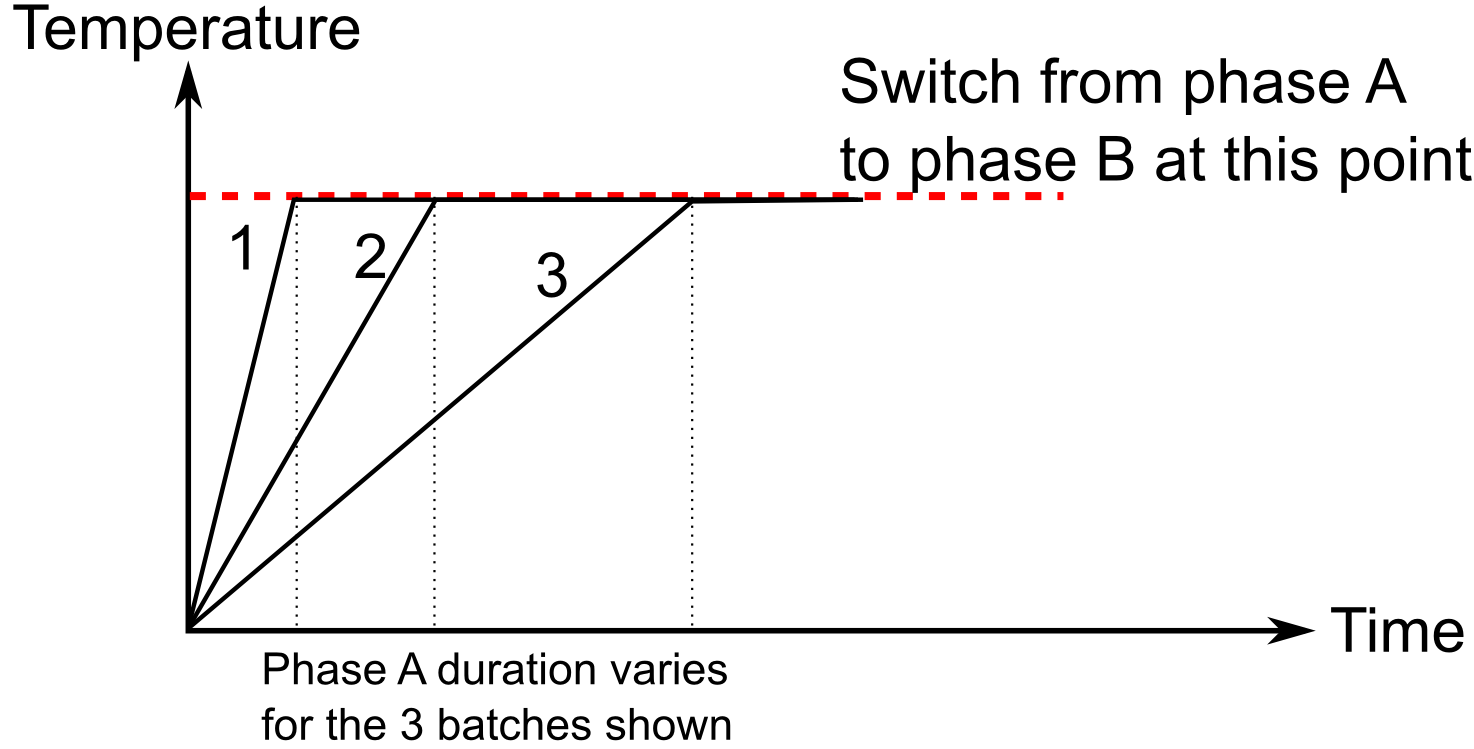
\includegraphics[width=0.7\textwidth]{images/alignment-due-to-phase-switching.png}
					\end{center}
		\end{itemize}
		\vspace{12pt}
		
	\column{0.3\textwidth}
	
		\begin{center}
			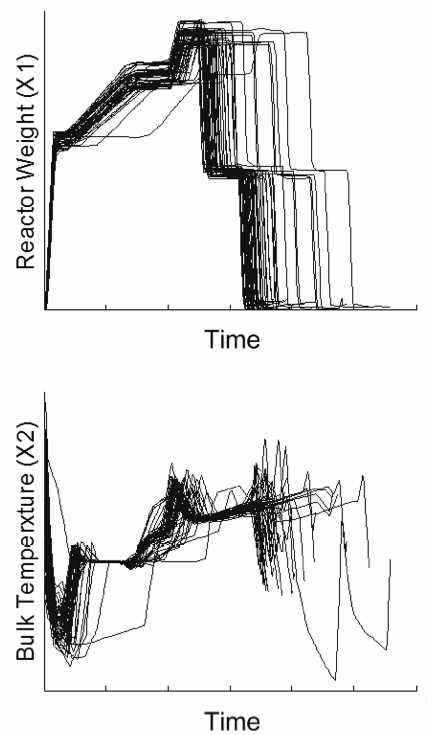
\includegraphics[width=\textwidth]{images/unaligned-trajectories-many-batches.png}
		\end{center}

		\small
		\textbf{Result}: similar trajectories of different duration
\end{columns}
\end{frame}

\begin{frame}\frametitle{Batch alignment: how to align}

Some automated tools are becoming available.  Best results still require case-specific knowledge.
\begin{itemize}
	
	\item	{\color{myGreen}{\emph{Data trimming}}}: throw out data points at start or end of each phase to match average duration.
	
			\begin{itemize}
				\item	\alert{Risk}:  most informative data often near start or end
			\end{itemize}
			
			\pause
	
	\item	{\color{myGreen}{\emph{Dynamic time warping}}}: stretch and shrink data to match a ``golden'' batch
	
			\begin{itemize}
				\item	Hard (impossible?) for real-time monitoring
			\end{itemize}
			
			\pause
	
	\item	{\color{myGreen}{\emph{Indicator variable}}}: find/create a monotonic variable within each phase and apply linear interpolation against it.
		
\end{itemize}

\end{frame}

\begin{frame}\frametitle{Batch alignment: aligning with an indicator}

\begin{itemize}
	
	\item	Good results if indicator is related to batch maturity
	
	\item	Adjust all other variables in phase against this indicator, and interpolate all batches to same number of \( J \) time points
	
	\item	Examples: 
			
			\begin{itemize}
				\item	temperature ramp
				
				\item	amount of raw material fed (semi-batch systems)
				
				\item	create a calculated variable, e.g. the total conversion
				
				\item	lance position in injection molding
			\end{itemize}
			
			\pause
	
	\item	Can be used for online, real-time monitoring (e.g. extrapolate temperature slope, use amount of material fed) \pause
	
	\item	Put the alignment information into \( Z \): very useful for diagnosis
\end{itemize}

\todo{Put some alignment diagrams from Cecilia's thesis here}

\end{frame}


% 
% %!TEX root = batch-course.tex
%-------------------------------------------------
\section{Final summary: learning from our data}
%-------------------------------------------------

\begin{frame}\frametitle{Value from batch process data}
\begin{enumerate}
	\item 	Learning more / confirming relationships
		
			\begin{itemize}
				\item 	understand between batch variation (overall scores, \( T^2 \), and SPE)
				\item 	understand within batch variation (instantaneous scores, \( T^2 \), and SPE)
			\end{itemize}
			
	\item 	Troubleshoot problems within a batch
	\item 	Optimize and improve: possible, but less likely in pharmaceutical applications
	\item 	Predictions: final quality attributes, endpoint
	\item 	Monitoring: can allow for early release to next stage
	
\end{enumerate}
\end{frame}


\end{document}

